
\singlespacing
\chapter{Wstęp}

\section{Od kodu kreskowego do znacznika radiowego}

Obserwujemy na przestrzeni ostatnich kulkudziesieciu lat znaczący rozwój technologii bezprzewodowej oraz mobilnych form płatności elektronicznej spowodował, że obecnie niemal na każdym kroku spotykamy się z systemami automatycznej identyfikacji (ang. \emph{Auto ID Systems}). Systemy te umożliwiają szybką, wygodną i bezbłędną identyfikacje produktów, sprzętu, ludzi a nawet zwierząt. Przekłada się to zazwyczaj na poprawę poziomu życia oraz jakości świadczonych usług spedycyjnych. Podstawowym zadaniem systemów automatycznej identyfikacji jest sprawne, przeprowadzone w czasie rzeczywistym i bez udziału człowieka, zarządzanie łańcuchem dostaw oraz kontrola jednostek logistycznych. Ostatnio systemy te coraz częściej wykorzystuje się do autoryzacji transakcji bankowych realizowanych za pośrednictwem sieci telefonii komórkowej, sieci przewodowej LAN i bezprzewodowej WLAN.


\noindent 
\newline Systemy automatycznej identyfikacji obejmują:
\begin{itemize}\setlength{\itemsep}{0pt}
    \item systemy kodów kreskowych (ang. \emph{bar code}),
    \item systemy kart elektronicznych (ang. \emph{electronic cards}),
    \item systemy RFID (ang. \emph{Radio Frequency Identyfication}),
    \item systemy automatycznego rozpoznawania pisma ręcznego ICR (ang. \emph{Intelligent Charakter Recognition}), 
    \item systemy automatycznego rozpoznawania znaków (druku) OCR (ang. \emph{Optical Character Recognition}),
    \item systemy biometryczne bazujące na technice:
	\begin{itemize}\setlength{\itemsep}{0pt}
		\item identyfikacji linii papilarnych,
		\item identyfikacji głosu,
		\item identyfikacji siatkówki oka,
		\item rozpoznawaniu twarzy
	\end{itemize}
\end{itemize}

Za protoplastę systemów automatycznej identyfikacji zwykło się uważać systemy kodów kreskowych wprowadzone do powszechnego użytku w latach 60-tych XX wieku.
Kod kreskowy nazywany często potocznie kodem paskowym (ang. \emph{bar code}) stanowi szereg ciemnych i jasnych pasków o zróżnicowanej szerokości wykorzystywanych do zakodowania danych cyfrowych. Wykorzystując własności optyczne nośnika informacji, w tym przypadku białej i czarnej farby tworzącej paski kodu kreskowego, jesteśmy w stanie szybko i w sposób jednoznaczny dokonać identyfikacyji skanowanego obiektu. Emitowane przez czytnik światło zostaje odbite od jasnych pasków, a pochłonięte przez paski czarne. Dekodowanie informacji cyfrowej zapisanej w kodzie kreskowym sprowadza się do porównania, mierzonego w luksach, natężenia światła emitowanego przez czytnik z natężeniem światła odbitego przez kod kreskowy. Zastosowanie odpowiedniego fotodetektora pozwala różnicę w poziomie natężenia światła przekształcić w ciąg impulsów elektrycznych, które są następnie przesyłane do komputera. W komputerze impulsy te są przetwarzane na ciąg odpowiednich znaków alfanumerycznych zapisywanych w bazie danych. 
Kody kreskowe są powszechnym i tanim sposobem etykietowania produktów. Zaletą tego systemu jest powszechna unifikacja sposobu kodowania, wadami natomiast możliwość zapisu małej ilości danych  oraz częsty problem z ich odczytem (dane trzeba wprowadzać ręcznie). Duży problem w wielu sytuacjach stanowi również niewielka wymagana odległość kodu od czytnika. 
Technologia kodów kreskowych jest obecnie najbardziej rozpowszechnioną i najtańszą technologią znakowania produktów, jednak osiągnęła już swoje granice możliwości – w pewnych zastosowaniach jest już niewystarczająca.
Coraz większą popularność zyskuje technika identyfikacji radiowej – \emph{RFID}. System jest bardzo prosty dzięki temu zyskuje na popularności zarówno przy dużych i kosztownych projektach, jak również w niewielkich przedsięwzięciach.

\section{Struktura systemu \emph{RFID}}

RFID (ang.\emph {Radio Frequency  Identyfication}) to jedna z najszybciej rozwijających  się automatycznych technologii bezprzewodowej  identyfikacji. Technologia ta umożliwia zdalne przechowywanie i odczytywanie danych z układów nazywanych znacznikami (ang. \emph{tag}) za pośrednictwiem fal radiowych. 

\noindent  
\newline W skład typowego systemu \emph{RFID} wchodzą następujące podzespoły:
\begin{itemize}\setlength{\itemsep}{0pt}

	\item znacznik  (etykieta, transponder, tag) –zbudowany z układu elektronicznego najczęściej microchipa z pamięcią, w którym dane są  kodowane i zapisywane w pamięci podręcznej oraz transmitowane za pomocą anteny nadawczo-odbiorczej (często napylanej na warstwie izolatora). Układ identyfikatora wykonany jest zazwyczaj na podłożu z papieru lub plastiku. 

	Etykiety \emph{RFID} mogą zawierać zarówno informacje zapisane w formie elektronicznej (pod postacią danych) jak również naniesiony tekst lub kod kreskowy. 

	Identyfikatory możemy sklasyfikować na dwa sposoby. W zależności od sposobu zasilania i sposobu zapisu danych. 

	\item czytnik - zbudowany z mikrokomputera, który weryfikuje poprawność otrzymanych informacji, modułu transmisji radiowej czyli nadajnika i odbiornika  odpowiedzialnych za odczyt i zapis danych w identyfikatorze oraz anteny lub cewki. Niektóre czytniki posiadają dodatkowo interfejs łączący z komputerem \emph{PC} (pozwalający na transmisję danych pomiędzy czytnikiem a komputerem).
	
	Oprogramowanie czytnika składa się z warstwy komunikacyjnej i użytkowej. Warstwa komunikacyjna odpowiedzialna jest za techniczną stronę transmisji danych, a warstwa użytkowa odpowiada za poprawne działanie aplikacji czyli wymianę, gromadzenie i przetwarzanie informacji na serwerze lub aplikacji klienckiej.


\end{itemize}



\section{Kryteria podziału znaczników i czytników}

\noindent 
Ze względu na sposób zasilania znaczniki dzielimy na: 
\begin{itemize}\setlength{\itemsep}{0pt}

	\item pasywne  (ang. \emph{passive}) (bez wewnętrznego zasilania), do zasilania  wykorzystują energię pozyskaną z pola elektromagnetycznego wytwarzonego przez czytnik, stanowią obecnie grupę najliczniej eksploatowanych znaczników, 

	\item aktywne (ang. \emph{active}) (z własnym źródłem zasilania np. baterią), emitują większy poziom mocy sygnału zwrotnego, pracują zazwyczaj na większych częstotliwościach przez co transmisja danych trwa krócej niż w innych znacznikach. Stosuje się je przede wszystkim do identyfikacji pojazdów,
	
	\item pół-pasywne (ang. \emph{semi-passive}), łączą cechy zarówno transponderów aktywnych jak i pasywnych. Transpondery te wyposażone są w baterię, która zasila obwód elektroniczny.Zasięg odczytu sięga 100 m, w dużym stopniu jednak zależy od czułości odbiornika w czytniku.  

\end{itemize}

\noindent 
\newline Ze względu na sposób zapisu danych znaczniki dzielimy na:
\begin{itemize}\setlength{\itemsep}{0pt}

	\item znaczniki typu \emph{RO} (ang.\emph{read only}) - tylko do odczytu – programowane podczas produkcji, zawierają numer seryjny (mogą zawierać również inne dane, których nie można modyfikować), 

	\item znaczniki typu \emph{RW} (ang.\emph{read write}) - do wielokrotnego zapisu i odczytu – zapisane dane mogą być wielokrotnie modyfikowane (pamięć może być podzielona na dwie części: część tylko do odczytu i część w której użytkownik może modyfikować zapisane dane),

	\item znaczniki typu \emph{WORM} (ang.\emph{write once read many}) - do jednokrotnego zapisu i wielokrotnego odczytu, część danych zapisana jest trwale, a część może być zmieniona przez użytkownika.

\end{itemize}


\noindent 
\newline Klasyfikacji czytników można dokonać według dwóch kryteriów - kryterium mobilności i kryterium komunikacji.



\noindent 
\newline Ze względu na na kryterium mobilności czytniki dzielimy na:

\begin{itemize}\setlength{\itemsep}{0pt}

	\item stacjonarne - pracujące w trybie autonomicznym – cały czas odczytuje etykiety znajdujące się w jego zasięgu, 

	\item interaktywne – w tym trybie komunikacja odbywa się za pomocą aplikacji pracującej na serwerze lub aplikacji klienckiej, 

	\item ruchome, przenośne.
\end{itemize}




\noindent
\newline Ze względu na typu interfejsu komunikacyjnego czytniki dzielimy na:

\begin{itemize}\setlength{\itemsep}{0pt}

	\item szeregowe - porty RS-232 lub RS-485, 

	\item sieciowe z interfejsem sieciowym np. Ethernet.

\end{itemize}



Technologia \emph{RFID} w ostatnim dziesięcioleciu zyskała miano jednego z najbardziej obiecujących i najprężniej rozwijających się systemów identyfikacji.
System \emph{RFID} pozwala na dużą automatyzację pracy zarówno podczas zapisu jak i odczytu danych. W przeciwieństwie do kodów kreskowych technologia ta nie wymaga bezpośredniej "widoczności" pomiędzy etykietą, a czytnikiem oraz daje możliwość odczytu wielu etykiet równocześnie.

%\newpage

\section{Zakresy częstotliwości}

Obecnie wdrażane systemy \emph{RFID} pracują na różnych zakresach częstotliwości, które można podzielić na następujące pasma:

\begin{itemize}\setlength{\itemsep}{0pt}
	\item pasmo niskich częstotliwości \emph {LF} (125-134.2 kHz).
Znaczniki \emph{LF} są zazwyczaj pasywne i mogą pracować w pobliżu elementów metalowych, substancji płynnych oraz innych elementów wykonanych z dobrych przewodników. Powoduje to, że znaczniki tego typu świetnie sprawdzają się jako identyfikatory narzędzi, podzespołów maszyn, pojazdów czy metalowych kontenerów. Znalazły również zastosowanie w rolnictwie do oznakowania zwierząt, leków oraz produktów spożywczych, gdyż fale elektromagnetyczne o niskiej częstotliwości wnikają w tkanki ciała i płyny.
Wygląd i budowa znaczników \emph{LF} zależy ściśle od ich przeznaczenia. Znaczniki używane jako immobilizery (elektroniczne zabezpieczenia przed niepowołanym uruchomieniem pojazdu) zazwyczaj wbudowane są w kluczyk natomiast cewka /  antena czytnika \emph{RFID} umieszczona jest współosiowo w stacyjce samochodu.
   
	\begin{figure}[h!]
	\centering
	    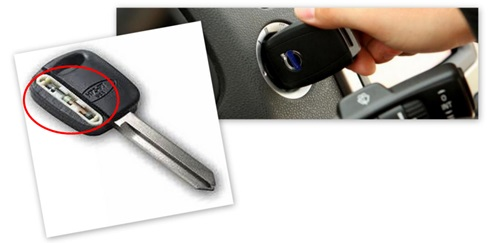
\includegraphics[width=9.32cm]{immobilizer.jpg}
	    \caption{Immobilizer samochodowy w technologii RFID}
	\end{figure}

	Dodatkowo systemy pracujące na częstotliwośći 135 kHz znalazły zastosowanie w automatycznej identyfikacji zwierząt hodowlanych i domowych.

	\begin{figure}[h!]
	\centering
	    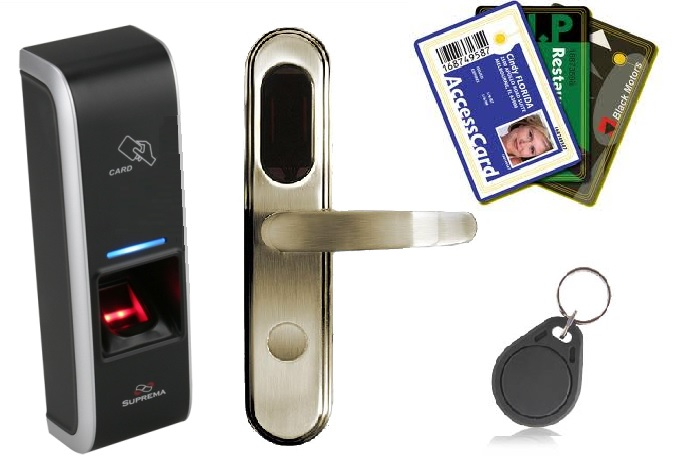
\includegraphics[width=7.27cm]{automatyczna_identyfikacja.jpg}
	    \caption{System kontroli dostępu bazujący na technologii RFID}
	\end{figure}
	
	\begin{figure}[h!]
	\centering
	    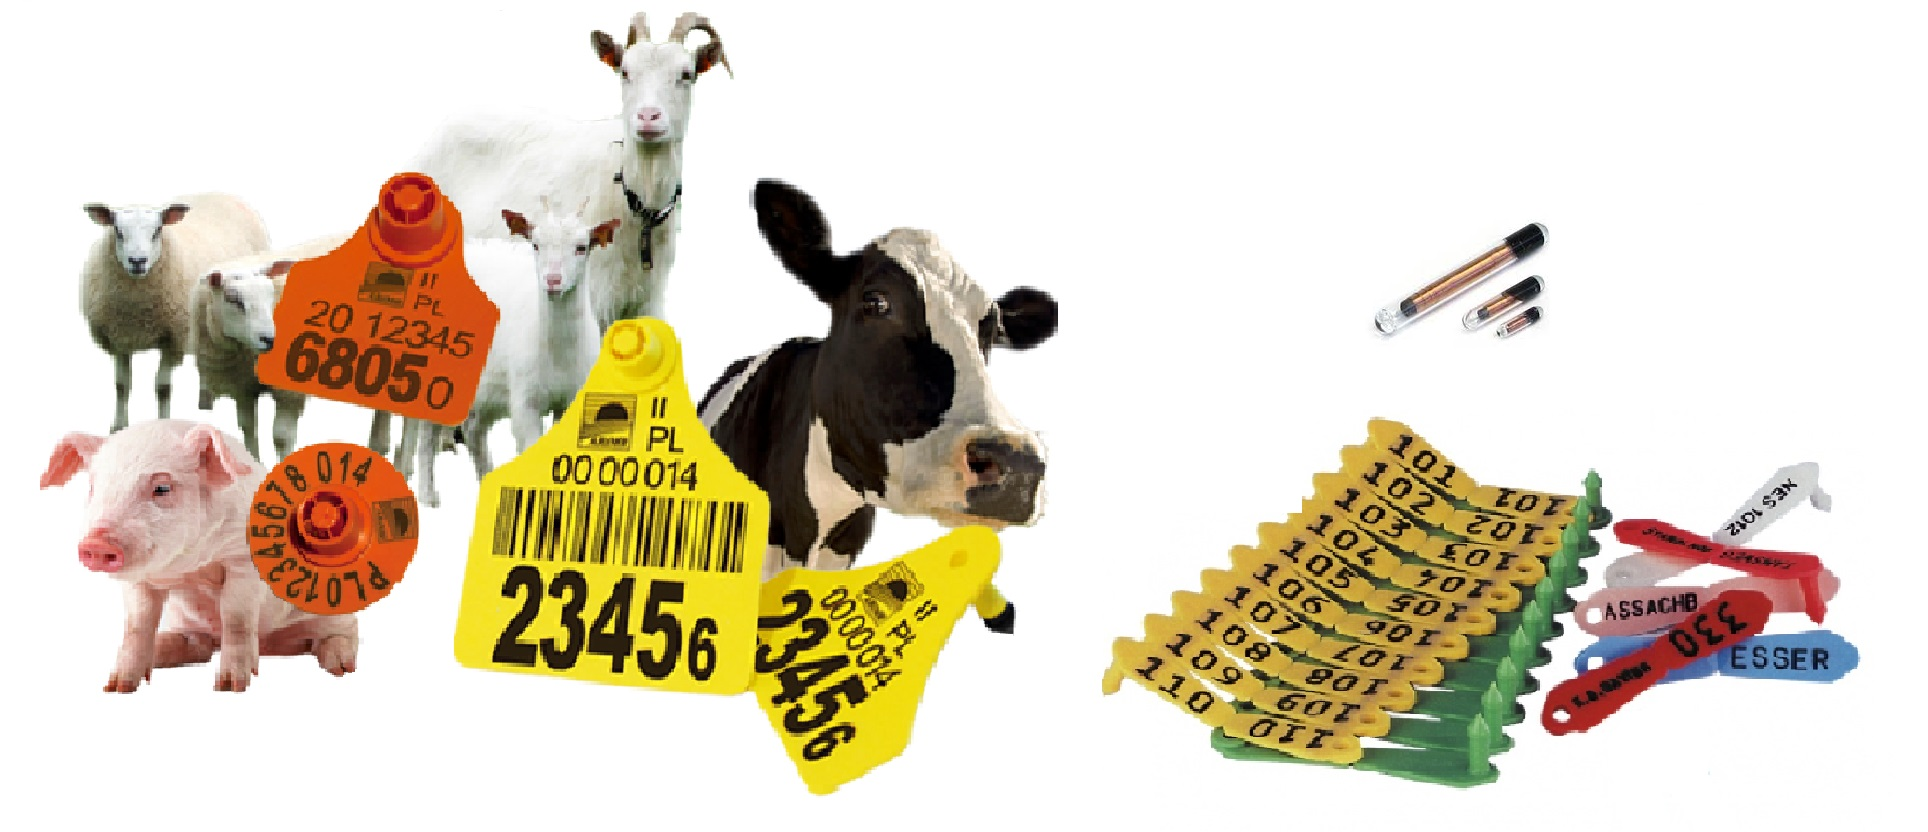
\includegraphics[width=14.34cm]{znakowanie_zwierzat.jpg}
	    \caption{Mikroczipy i kolczyki stosowane do znakowania zwierząt oraz kapsułki (biochipy) do wszczepiania pod skórę}
	\end{figure}
	
	Znaczniki LF zbudowane są z ferrytowego rdzenia, na którym nawinięte są zwoje cewki. Występują w formie plastikowych kart, krążków, biochipów, pastylek. Wadami systemu \emph{RFID-LF} są: mała szybkość transmisji danych (1-2 kb/sek), co znacznie ogranicza możliwą do zapisania / odczytania ilość danych, niewielki zasięg – około 0.5 metra, podatność na zakłócenia przez urządzenia elektryczne, co ogranicza zastosowanie w przemyśle, limit jednoczesnego odczytu nie więcej niż 20 transponderów co ogranicza to pojemność systemu i maksymalną liczbę odczytów jaką może obsłużyć jeden czytnik. 

	\newpage


	\item pasmo wysokich częstotliwości \emph{HF} (częstotliwości 6.78 MHz, 13.56 MHz, 27.125 MHz oraz 40.68 MHz). 
Transpondery \emph{HF} pracujące w zakresie 13.553 MHz – 13.657 MHz to zazwyczaj znaczniki pasywne. Identyfikatory pracujące na wysokich częstotliwościach wykazują większą wrażliwość na obecność w swoim otoczeniu metali i mniejszy wpływ na zakłócenia elektromagnetyczne pochodzące od innych urządzeń niż znaczniki \emph{LF}. Pamięć znaczników \emph{HF} ma kilka razy większą pojemność, a szybkość komunikacji sięga 20 kbit/s. Cewka transpondera \emph{HF} zbudowana jest zazwyczaj z 3-8 zwojów, nadrukowanych za pomocą przewodzącego lakieru na podłoże i zaprasowanych w etykiecie. Znaczniki te produkowane są w postaci samoprzylepnych etykiet (ang.\emph{smart label}). Zaletami transponderów \emph{HF} są znacząco mniejsze koszty wykonania w porównaniu z identyfikatorami \emph{LF}, co spowodowane jest niewielką grubością identyfikatora, która osiąga nawet 0,1 mm. System RFID-HF daje możliwość odczytu do 50 znaczników jednocześnie (dzięki wprowadzeniu mechanizmów antykolizyjnych), co pozwala zastosować je do automatycznej identyfikacji produktów i obiektów. System wymaga zachowania odległości co najmniej 2-3 centymetrów pomiędzy transponderami. 
	
	Typowo zasięg działania systepu RFID pracującego w paśmie HF wynosi 1-1.5 metra. Można uznać to za zaletę w przypadku systemu typu PayPass (płatności zbliżeniowe). Właściwość ta dodatkowo podnosi poziom bezpieczeństwa całego systemu, zmniejszając liczbę prób nieautoryzowanego dotępu.  

	\begin{figure}[h!]
	\centering
	    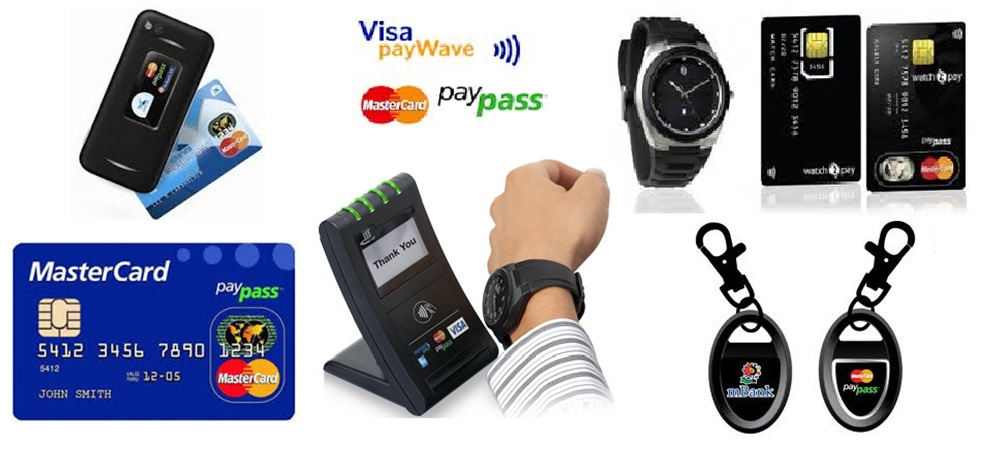
\includegraphics[width=16.56cm]{karty_platnicze.jpg}
	    \caption{Karty i breloki systemu PayPass}
	\end{figure}

	Systemy \emph{HF} są popularne ponieważ posiadają możliwość wielokrotnego zapisu danych, która jest niezbędna zarówno przy znakowaniu książek, dokumentów (paszportów, legitymacji studenckich, biletów komunikacji miejskiej, kart płatniczych) jak i bagażu na lotnisku, czy odzieży w pralni.

	\begin{figure}[h!]
	\centering
	    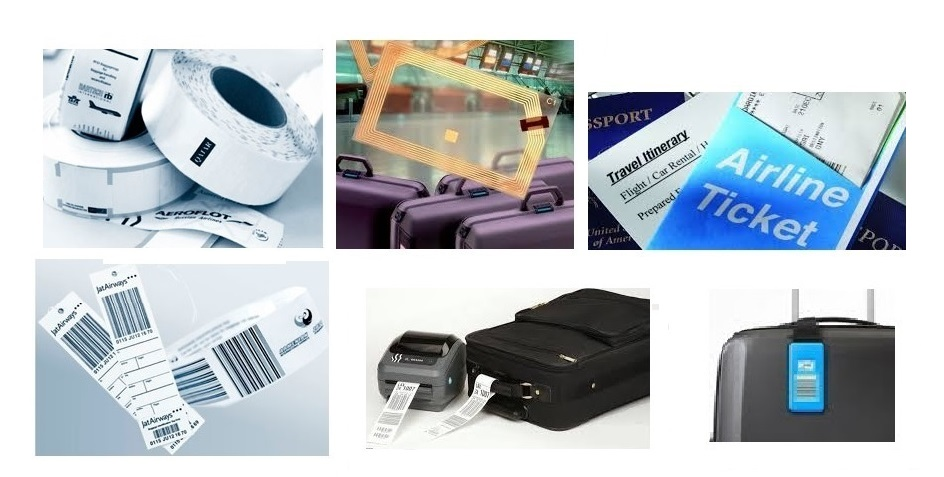
\includegraphics[width=15.51cm]{bagaz.jpg}
	    \caption{Znakowanie bagażu lotniczego}
	\end{figure}

	\begin{figure}[h!]
	\centering
	    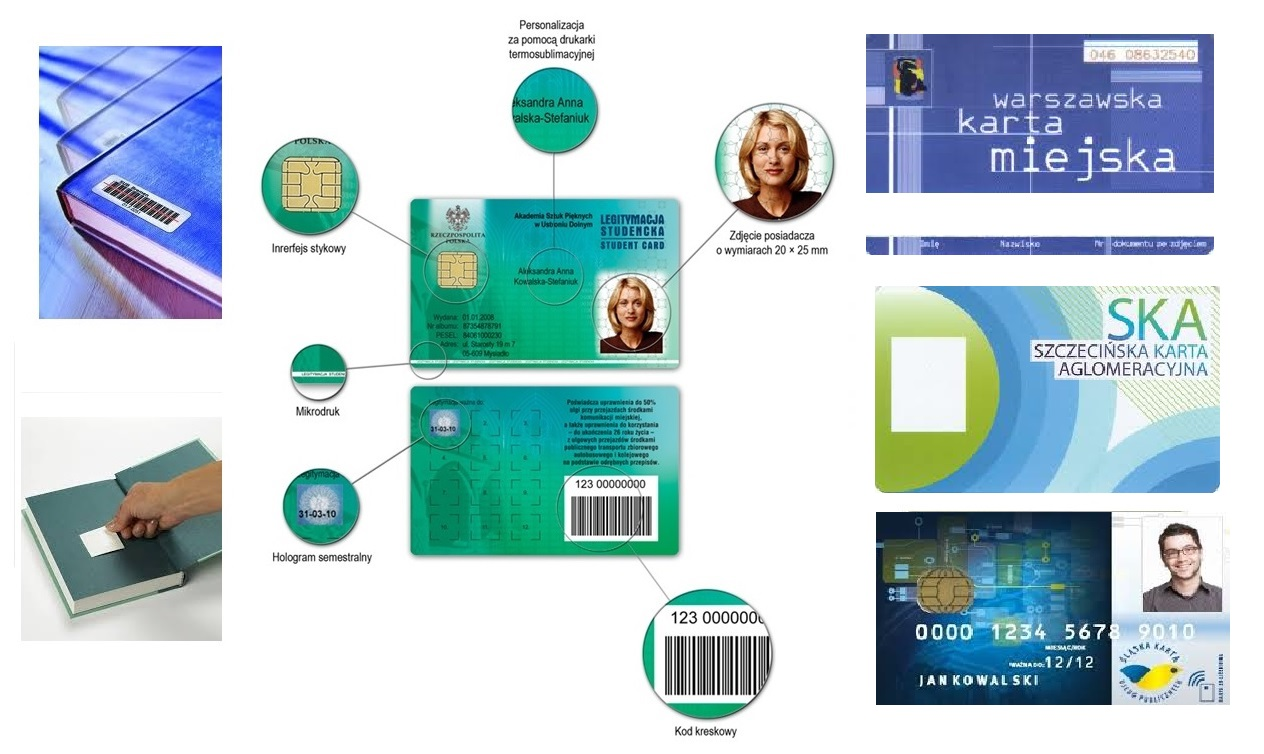
\includegraphics[width=16.82cm]{dokumenty.jpg}
	    \caption{Znakowanie książek, dokumentów, kart miejskich}
	\end{figure}
	
	 System znaczników pracujących na wysokich częstotliwościach znalazł zastosowanie w Europejskim Systemie Sterowania Pociągiem (ang. \emph{ETCS - European Train Control System}). System ten wyposażony w jest w urządzenie zwane Eurobalisą, które mocowane jest na torze pomiędzy szynami i może komunikować się z przejeżdżającymi nad nim pociągami.

	\item pasmo ultra wysokich częstotliwości \emph{UHF} (częstotliwości 433.92 MHz i 860-960 MHz).
Zakresy częstotliwości \emph{UHF} podzielono na kilka podzakresów np. Europa 860-868 MHz, Ameryka Północna 902-928 MHz, Japonia  950 MHz-956MHz. W związku z różnicami w częstotliwościach pracy urządzeń ustalono globalny standard ISO/IEC 18000-6 C. W celu objęcia globalnego łańcucha dostaw stworzono identyfikatory i czytniki, które mogą pracować na całym świecie. Znaczniki pasywne systemów \emph{RFID} pracujące w pasmie \emph{UHF} pozwalają na dużo większy zasięg niż znaczniki pasywne pozostałych pasm częstotliwości. Zaimplementowano lepsze protokoły antykolizyjne niż w systemach \emph{HF}. Wskutek tego osiągnięto się możliwość odczytu do 200 znacznikóa jednocześnie. Zasięg odczytu zawiera się w granicach od 3 do 6 metrów.Dodatkowo duża szybkość transmisji danych do 120 kbit/sek powoduje, że znajdują one zastosowanie w magazynach.

Podobnie jak znaczniki \emph{UHF} nie mogą być używane w pobliżu elementów metalowych, substancji płynnych i innych dobrych przewodników. 
Znaczniki \emph{UHF} ze względu na duży zasięg bardzo często stosowane są do śledzenia obiektów w logistyce. Wiele firm logistycznych, handlowych i spedycyjnych używa tylko i wyłącznie znaczników pasywnych \emph{UHF} ze względu na bardzo niski koszt produkcji, wynoszący kilkanaście groszy. 
Częstotliwość \emph{UHF} jest najbardziej rozpowszechnioną częstotliwością w logistyce i produkcji.

	\begin{figure}[h!]
	\centering
	    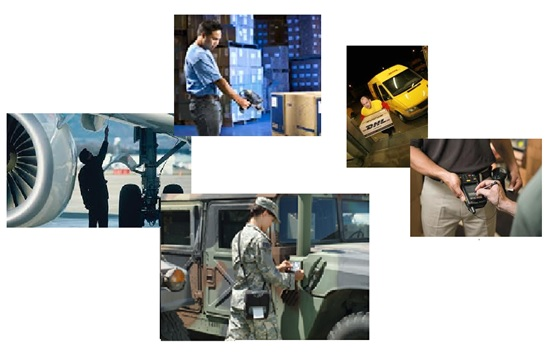
\includegraphics[width=14.37cm]{logistyka_transport_przemysl.jpg}
	    \caption{Przykłady zastosowań systemów RFID-UHF w sektorze logistyki, produkcji, transportu i handlu}
	\end{figure}

	\item pasmo mikrofalowe \emph{MW} (częstotliwości to 2.45 GHz, 5.8 GHZ i 24.125 GHz).
W paśmie \emph{MW} wykorzystuje się w większości znaczniki aktywne lub pasywno-aktywne. Są  mniejsze niż znaczniki pracujące na innych pasmach częstotliwości jednak droższe. Zasięg odczytu dochodzi do kilkuset metrów. Najistotniejszą zaletą tagów pracujących na częstotliwości mikrofalowej okazuje się wysoki transfer danych, który  umożliwia odczyt informacji z obiektów poruszających się z prędkością ponad 100 km/h, co nie jest możliwe w technologii znaczników \emph{LF} i \emph{HF}. Pozwala to na wykorzystanie ich do identyfikacji środków transportu komunikacji miejskiej, samochodów poruszających się  na autostradzie (automatyczne naliczanie opłaty za przejazd autostradą), rejestracji przejeżdżających pociągów, czy statków.

	\begin{figure}[h!]
	\centering
	    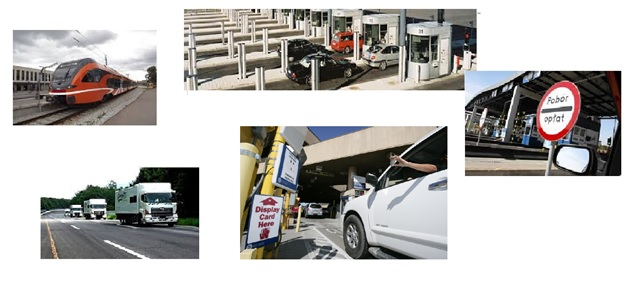
\includegraphics[width=16.61cm]{autostrady.jpg}
	    \caption{Naliczanie opłat za przejazd autostradą oraz identyfikacja środków komunikacji miejskiej}
	\end{figure}

	Znaczniki pracujące na częstotliwości 5.8 GHz montowane są w czujnikach przed drzwiami (w sklepach i marketach), w czujnikach ruchu jak również w systemach automatycznego spłukiwania toalet.
	Jedną z wad znaczników \emph{MW} jest możliwość wystąpienia zjawiska interferencji, które zakłóca  transmisję w środowisku o dużym zagęszczeniu znaczników jak również spowoduje zakłóca w działaniu systemów pracujących  w pobliżu substancji płynnych lub metali.

\end{itemize}

\newpage

\section{Główne obszary zastosowania systemów \emph{RFID}}

\noindent 
Technologia \emph{RFID} znalazła zastosowanie w niżej wymienionych sektorach gospodarki: 

\begin{itemize}\setlength{\itemsep}{0pt}
	\item logistyka, transport i magazynowanie – w przypadku konieczności szybkiej identyfikacji i śledzenia poszczególnych elementów łańcucha dostaw. Identyfikacja i rejestracja towarów w magazynie i na kolejnych etapach produkcji / dystrybucji.  Śledzenie przesyłek pocztowych / kurierskich, bagaży na lotnisku.  Znaczniki \emph{RFID} stopniowo wypierają etykiety logistyczne i kody kreskowe,

	\item płatności elektroniczne– systemy płatnicze PayPass, systemy kart rabatowych w hipermarketach i na stacjach benzynowych, 

	\item elektroniczne bilety, karty wstępu – komunikacja miejska, imprezy masowe/imprezy sportowe, opłaty za przejazd autostradami, systemy \emph{skipass},

	\item organizacja pracy – kontrola dostępu do wyznaczonych miejsc poprzez umieszczanie znaczników \emph{RFID} w identyfikatorach (np. kartach, breloczkach). Pozwalają one na identyfikację właściciela, monitoring czasu pracy oraz system kontroli dostępu (inteligentne budynki),

	\item znakowanie zbiorów, odzieży – archiwa, muzea i biblioteki w których na książkach coraz częściej zamiast kodów kreskowych znajdują się znaczniki RFID, które ułatwiają identyfikacje jak również zabezpieczają przed kradzieżą. Znakowanie odzieży w celu rozpoznawania i sortowania m.in. pralniach jak i w sklepach również w celu ochrony przed kradzieżą jak i fałszerstwem produktów markowych,
 	
 	\item dokumenty, papiery wartościowe– znaczniki w postaci samoprzylepnych etykiet. Śledzenie i zapisywanie historii obiegu oraz aktualnej lokalizacji ważnych dokumentów.  W paszportach stosowane w celu przechowywania danych osobowych oraz informacji na temat przekraczanych granic. Wymagane zabezpieczenie przed odczytem danych przez niepowołane osoby,
	
	\item przemysł – oznaczanie i  identyfikacja podzespołów, półproduktów oraz zapis poszczególnych stanów procesów produkcyjnych, co pozwala na ich automatyzację. Śledzenie obiektów na liniach produkcyjnych, rejestracja danych, identyfikacja cystern, wagonów pojemników w procesie produkcji
	
	\item dane eksploatacyjne maszyn – identyfikacja tonerów do drukarek tak, aby drukarki nie podejmowały pracy w momencie przekroczenia dopuszczalnej liczby wydrukowanych stron na jednym tonerze lub w przypadku gdy toner nie pochodzi do konkretnego producenta, 
	
	\item rolnictwo, znakowanie zwierząt hodowlanych, zagrożonych gatunków – oznakowanie zwierząt za pomocą znaczników występujących w postaci charakterystycznych żółtych klipsów przymocowywanych do uszu bydła i trzody chlewnej. Pozwalają na identyfikację zwierząt, a co za tym idzie odczytanie m.in. miejsca ich chowu,
	
	\item sport – rejestrowanie czasów oraz ilości okrążeń w zawodach sportowych. 
	
	\item transpondery na oponach samochodowych – zawierają najczęściej numer identyfikacyjny, datę produkcji oraz stopień zużycia opony.

\end{itemize}


\section{Wykorzystanie technologii \emph{RFID} w różnych sektorach gospodarki}

	\begin{figure}[h!]
	\centering
	    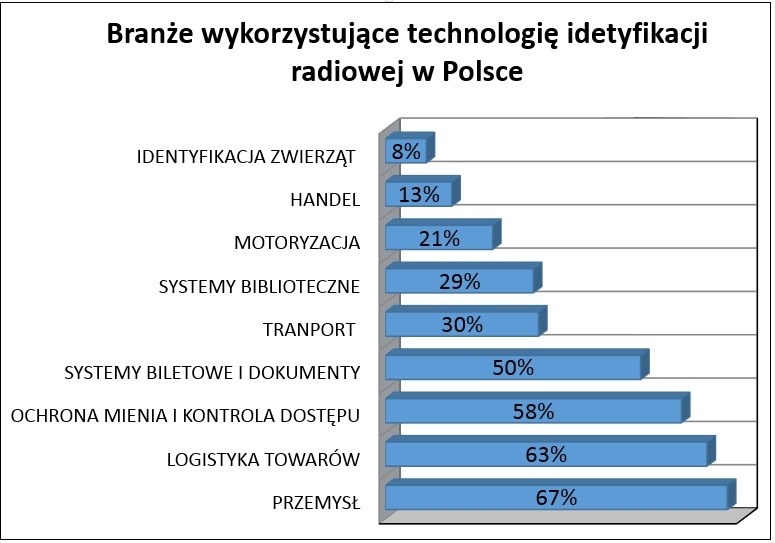
\includegraphics[width=16.2cm]{wykres_ver3.jpg}
	    \caption{Procentowy udział branż wykorzystujących technologię \emph{RFID}}
	\end{figure}


\section {Zalety i wady zastosowania systemu \emph{RFID}}

\noindent 
Zalety technologii \emph{RFID}:

\begin{itemize}\setlength{\itemsep}{0pt}
	\item nie jest wymagany optyczny kontakt zarówno przy zapisie jak i odczycie czytnika z identyfikatorem, dzięki temu operację ta można zautomatyzować i zrealizować szybciej,
	
	\item możliwość odczytu wielu identyfikatorów równocześnie,
	
	\item duża pojemność pamięci, możliwość przechowywania większej ilości danych niż w przypadku kodów kreskowych

	\item możliwość aktualizacji / zmiany, wielokrotnego zapisywania i dopisywania danych  na etykiecie,

	\item identyfikatory mogą być wykorzystane wielokrotnie,

	\item duża prędkość transmisji danych,

	\item możliwość zapisywania danych w trakcie ruchu obiektu,

	\item duże bezpieczeństwo danych -istnieje możliwość zastosowana różnych metod ochrony danych zapisanych w znaczniku, zabezpieczenie dostępu do pamięci, zabezpieczenie dostępu hasłem,  

	\item miniaturyzacja znacznika - najmniejszy wyprodukowany na świecie znacznik przez firmę Hitachi posiada wymiary 0,05 x 0,05 mm

	\item możliwość pracy w trudnych warunkach przemysłowych w miejscach, gdzie występuje duże zapylenie, bardzo wysokie lub bardzo niskie ciśnienie, niska temperatura, agresywne środowisko chemiczne np. kopalnie, zakłady przemysłowe, chłodnie itp.

	\item możliwość integracji z istniejącymi systemami automatycznej identyfikacji (kody kreskowe),

	\item możliwość wykorzystania tych samych identyfikatorów w całym łańcuchu dostaw.

\end{itemize}

\noindent 
\newline Wady technologii \emph{RFID}:


\begin{itemize}\setlength{\itemsep}{0pt}

	\item brak jednolitego standardu dla protokołu RFID,
	
	\item możliwość zakłócenia przez odziaływanie elektromagnetyczne, wilgoć czy metale,
 	
 	\item większy koszt pojedynczego znacznika, w porównaniu z kodem paskowym, zwłaszcza w przypadku znaczników o większej funkcjonalności 

\end{itemize}





\chapter{Technologia anten konforemnych}

Układy antenowe o elastycznych, giętkich podłożach są trudne technologicznie do wykonania jednak mają szerokie zastosowanie praktyczne ze względu na możliwosć kształtowania powierzchni. 
W trakcie realizacji konforemne anteny i układy antenowe sprawiają wiele problemów konstrukcyjnych, gdyż nawet małe deformacje i odkształcenia mają duży wpływ na ich parametry polowe. 
Anteny konforemne dają możliwość uzyskania szerszego pokrycia kątowego płaszczyzny skanowania. Celem uzyskania poprawnych charakterystyk promieniowania należy w trakcie projektowania takich anten uwzględnić zmiany amplitud i faz sygnałów otrzymanych na poszczególnych elementach promieniujących, będących wynikiem chociażby odkształcenia ich struktury.    
Metody projektowania i konstruowania anten są na tyle skomplikowane, że cały proces łącznie z badaniami, aż do praktycznej realizacji przebiega z udziałem grupy sapecjalistów z różnych dziedzin (kompatybilności elektromagnetycznej, technologii materiałowych, systemów tekstronicznych, radioelektroniki, telekomunikacji, przetwarzania sygnałów i innych). Anteny o elastycznej strukturze przeznaczone są głównie do wykorzystania w pasmie powyżej 1 GHz.     

\section{Obszary wykorzystania i zastosowania anten konforemnych}

Możliwości zastosowania tego typu anten jest wiele. Dziedziny zastosowań wzajemnie się przenikają i uzupełniają, jednak można wyróżnić trzy najbardziej rozpowszechnione zastosowania, do których należą:

\begin{itemize}\setlength{\itemsep}{0pt}
	
	\item zastosowania medyczne - radary przenzaczone do mocowania na skórze: sportowców, ratowników medycznych, strażaków, żołnierzy. Czujniki służą do monitorowania aktywności (rytmu serca, oddechu) i stanu fizjologicznego człowieka (poziomu wydzielanego potu, stężenie tlenu i dwutlenku węgla we krwi, stanu odwodnienia, poziomu elektrolitów).Przekazywanie informacji o parametrach życiowych (np.temperaturze ciała). Wykrywanie zewnętrznych zagrożeń np. stężenie niebezpiecznych substancji chemicznych, gazów, oparów. Możliwość zaastosowana do wykrywania komórek nowotworowych,  

\begin{figure}[h!]
\centering
	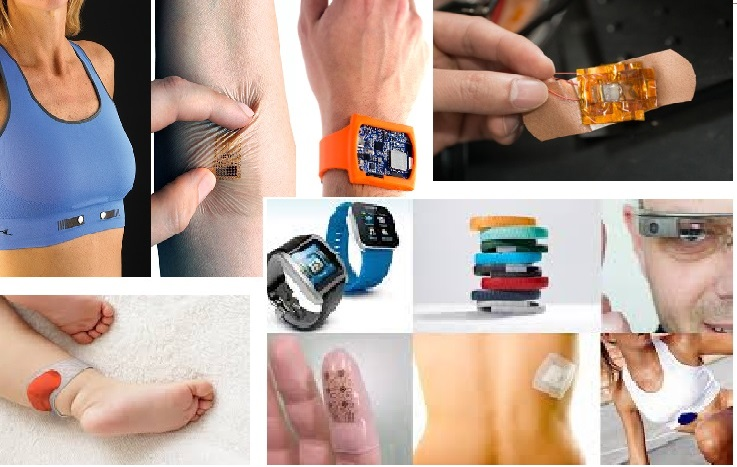
\includegraphics[width=14cm]{anteny_konforemne.jpg}
	\caption{Przykłady zastosowań anten konforemnych}
\end{figure}

	\item zastosowania militarne - system lokalnych sieci WBAN, wspieranie systemów rozpoznawania terenu UAVs (mobilny system łącznosci), określanie lokalizacji np. żołnierza, maskowanie aparatury do łączności.
	Zastapienie kilku urządzeń monitorujących systemem anten, a więc zmniejszenie wagi potrzebnego sprzętu. Zwiększenie niezawodności łączności (z ratownikami medycznymi, żołnierzami), a co za tym idzie poprawa mobilności służb,      

	\item zastosowanie to tworzenia krótkodystansowych systemów łączności bezprzewodowej - zastsowanie w sieciach: \emph{WPAN} (ang.\emph{Wireless Personal Area Network}), \emph{WBAN} (ang. \emph{Wireless Body Area Network}) oraz \emph{UWB} (ang. \emph{Ultra WideBand}). Współpraca czujników wszytych w ubranie (monitorowanie oznak życia organizmu). Integracja anten z elementami wyposażenia: kamizelką, rękawem, kołnierzem, hełmem (np. strażaka, żołnierza, policjanta) przy wykorzystaniu technologii Bluetooth, standardów GSM lub UMTS. Kominikacja anten z urzadzeniami działającymi w sieciach Wireless USB, Bluetooth, WLAN.  

\end{itemize}
	

\section{Częstotliwosci pracy dla anten konforemnych}
 
\noindent Pasma pracy:

\begin{itemize}\setlength{\itemsep}{0pt}
	
	\item UWB/WUSB: 3.1GHz - 10.6 GHz (FCC) - pasmo stosowane w systemach łączności krótkodystansowej, bazujące na przesyłaniu ultra-krótkich impulsów,

	\item ISM: 2.4 GHz - 2.4835 GHz - zakres używany przede wszystkim dla systemów łączności krótko i średniodystansowych takich jak Bluetooth, sieci WLAN / WBAN / WPAM,

	\item GPS: L1: 1575.42 MHz, L2: 1227.6 MHz, Galileo: 1176.45 MHz - częstotliwość pracy wykorzystywana do nawigacji satelitarnych GPS, Galileo i innych oraz do współpracy Galileo z innymi systemami takim jak GPS, Glonass, Loran-C, UMTS.

	\item ZigBee: 868 MHz, 915 MHz, 2.4 GHz - częstotliwości te znalazły zastosowanie w tworzeniu bezprzewodowych sieci sensorycznych.

	\item Zastosowania militarne: 50-300 MHz pasamo pracy przeznaczone dla radarów przenośnych oraz kamizelek z zintegrowanymi systemami łączności (antenami).

\end{itemize}

\section{Anteny tekstylne}

Tekstronika jest nową gałęzią nauki, zajmującą się projektowaniem i budową inteligentnej odzieży. Jest wynkiem połączenia kilku dziedzin nauki m.in. nauki o materiałach, włókiennictwa, elektroniki, radiokumunikacji, kompatybilności elektromagnetycznej jak również informatyki. Tekstronika stwarza możliwość wykorzystania różnych metod transmisji sygnałów w układach antenowych (patrz Rys. 2.2). W ramach niniejszej pracy skoncentrowano się na transmisji bezprzewodowej w paśmie nielicencjonowanym 2.4 GHz - 2,4835 GHz.  
Anteny do zastosowań tekstronicznych, czyli implementowane w odzieży, dzięki eleastycznej i giętkiej konstrukcji są łatwe do integracji z materiałami.


\begin{figure}[h!]
	\centering
	    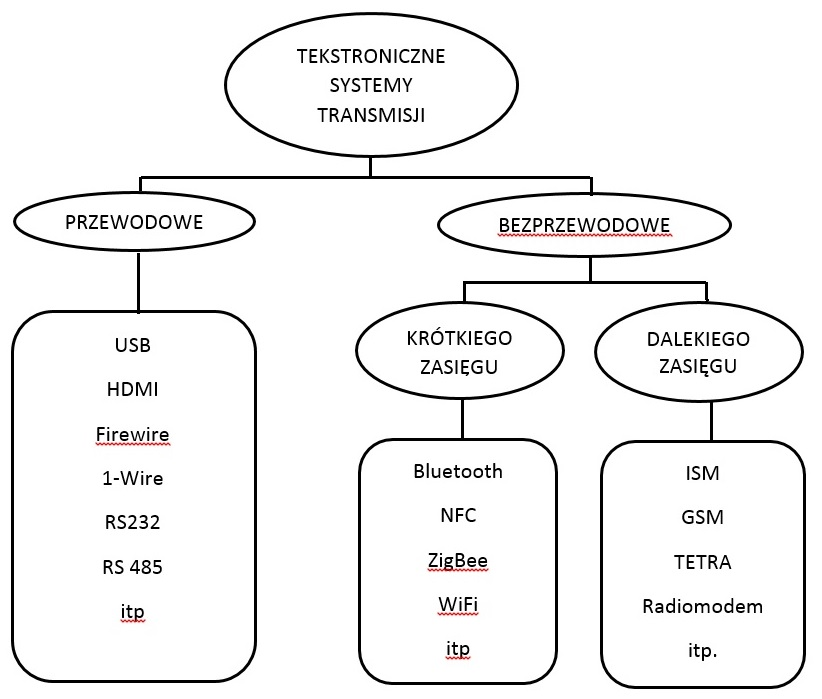
\includegraphics[width=15.5cm]{diagram.jpg}
	    \caption{Podział tekstronicznych systemów transmisji}
\end{figure}


 \chapter{Cel i zakres pracy}

Celem niniejszej pracy było zaprojektowanie i wykonanie anteny tekstylnej przewidzianej do pracy w paśmie \emph{ISM} (2.4 GHz). 
Praca nad projektem inżynierskim przebiegała w kilku etapach:

\begin{itemize}\setlength{\itemsep}{0pt}
	
	\item stworzenie modelu symulacyjnego badanej anteny,

	\item symulacje zaproponowanej struktury anteny,

	\item przeprowadzenie analizy numerycznej,

	\item wykonanie modelu i pomiar wybranych parametrów anteny.

\end{itemize}

Wszystkie symulacje numeryczne przeprowadzone zostały w srodowisku \emph{CST Microwave Studio}. Program umożliwia zaprojektowanie i przeprowadzenie dokładnych symulacji prototypu anteny.


\chapter {Projekt anteny}

\section{Wstęp}

\noindent Najważniejsze parametry anten, które należy wziąć pod uwagę w procesie ich projektowania:

\begin{itemize}\setlength{\itemsep}{0pt}

	\item pasmo pracy - czyli zakres częstotliwości, dla których projektowana antena spełnia założone wcześniej kryteria. Pasmo pracy anteny powinno być możliwie szerokie - dla anten RFID nie powinno jednak przekraczać 30 MHz,

	\item ipedancja wejściowa - jest to stosunek napięcia do natężenia prądu na zaciskach wejściowych anteny. Na impedancję wpływa obecność innych anten lub obiektów znajdujących się w pobliżu.
	Standardowa impedancja linii transmisyjnych wynosi 50\(\Omega\),

	\item zysk energetyczny - defionowany jako zysk kierunkowy zględem anteny wzorcowej (anteny izotropowej).
	Jest to stosunek gęstości mocy promieniowania w danym kierunku do średniej gęstości mocy wypromieniowanej przez antenę w pełnym kącie bryłowym. Podawany zazwyczaj dla kierunku, w którym promieniwanie anteny jest najsilniejsze, 

	\item charakterystyka promieniowania - pokazuje w jaki sposób antena promieniuje energię w różnych kierunkach. Obrazuje unormowany rozkład pola elektrycznego. Charakterystyka może być wyznaczona w dwóch płaszczyznach lub mieć postać trójwymiarową,

	\item polaryzacja anteny - określa ją polaryzacja wytwarzanej przez nią fali elektromagnetcznej 
	Wyróżniamy polaryzację liniową (pionową, poziomą, nachyloną pod kątem), eliptyczną lub kołową ( lewoskrętną, prawoskrętną),

	\item kierunkowość - to silna koncentracja energii anteny w jednym kierunku, kosztem innych kierunków. Kierunek, w którym promieniowanie anteny jest największe nazywamy kierunkiem maksymalnego promieniowania,

	\item sprawność - to storunek mocy wypromieniowanej przez antenę do mocy dostarczonej do anteny,

	\item dopasowasowanie - linia transmisyjna jest dopasowana gdy impedancja wejściowa linii równa jest impedancji wejsciowej anteny. 

\end{itemize}

\newpage
\section{Struktura anteny}

Prototyp anteny tekstylnej RFID przesymulowano w środowisku \emph{CST Microwave Studio}. Źródłem inspiracji była struktura zamieszczona w artykule z KKRRiT z 2013 roku \cite{Artykul_1}. Strukturę bazową poddano modyfikacji celem dostosowania do założeń projektu. Parametry symulacji optymalizowano poprzez wybór opcji \emph{adaptive mesh refinement}, która ma na celu dostosowanie rozmiaru siatki oraz parametryzację struktury dzięki czemu otrzymane wyniki są dokładniejsze.

\begin{figure}[h!]
\centering
	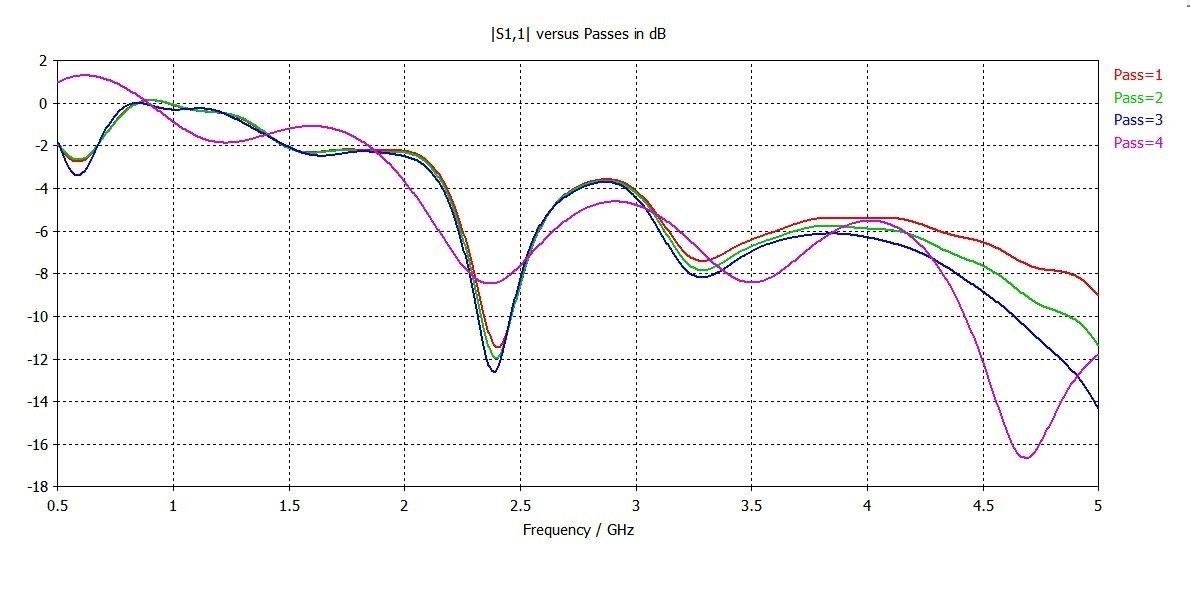
\includegraphics[width=17cm]{S11_Passes_dB.jpg}
	\caption{Wykres przedstawia analizę doboru rozmiaru siatki pod kątem parametru $s_{11}$}
\end{figure}

\begin{figure}[h!]
	\centering
	    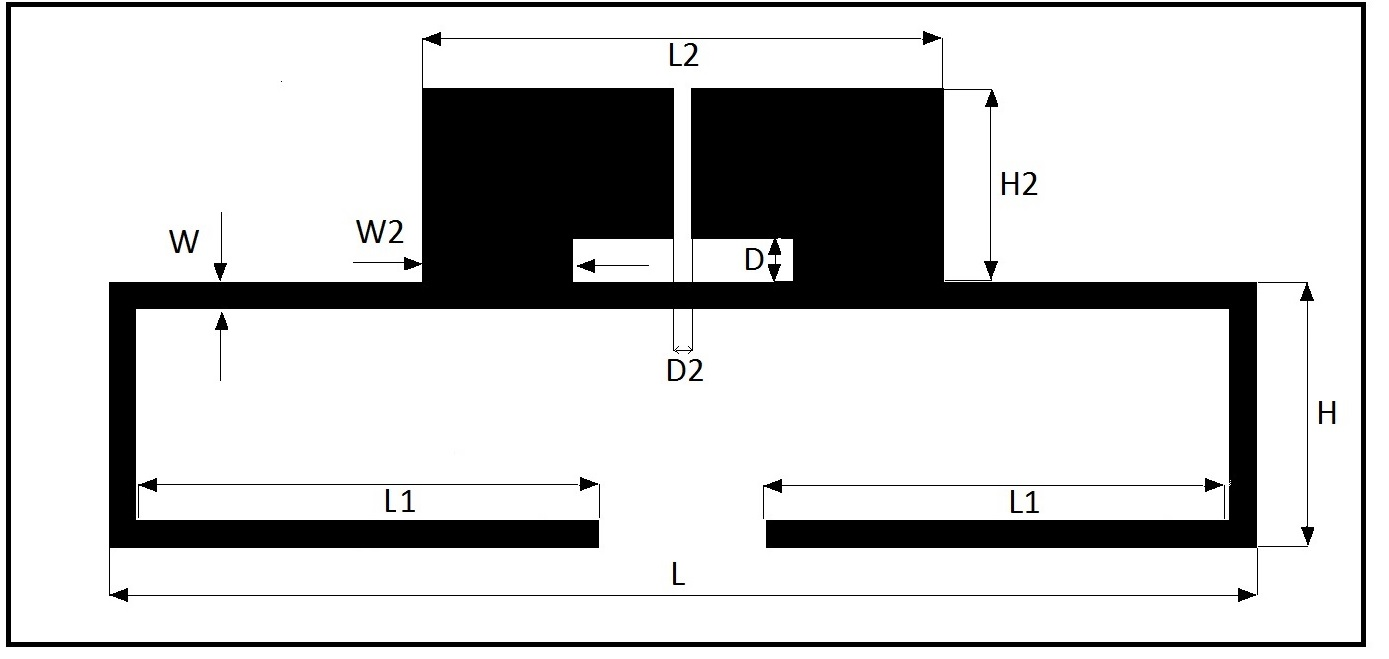
\includegraphics[width=15.5cm]{struktura.jpg}
	    \caption{Model struktury anteny}
\end{figure}

\begin{figure}[h!]
	\centering
	    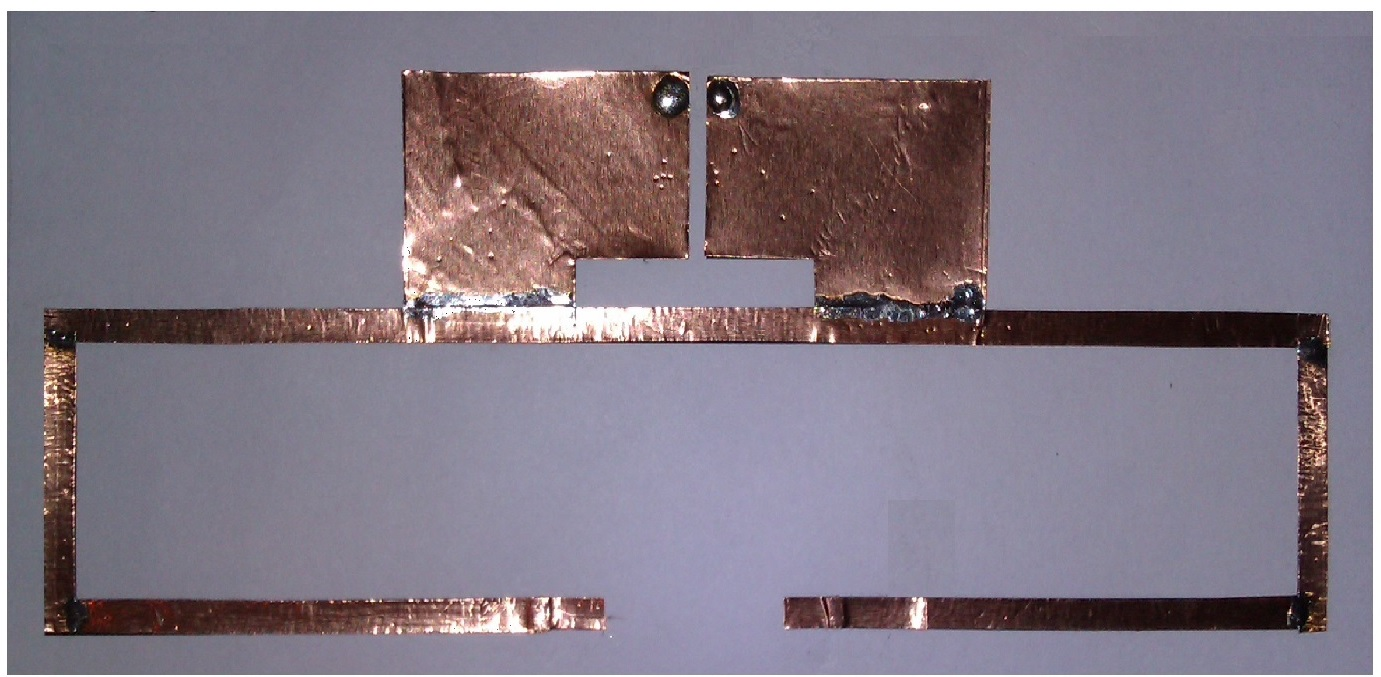
\includegraphics[width=15.5cm]{fizyczna_antena.jpg}
	    \caption{Prototyp anteny}
\end{figure}

\newpage
 Stopień dyskretyzacji został ustalony po 6 iteracjach. Rezultaty procesu doboru wymiarów anteny, można było obserwować na wykresach. Najlepsze wyniki posłużyły do ustalenia rozmiaru projektowanej anten, a pózniej wykonania prototypu. Schemat struktury po parametryzacji i prototyp pokazano na Rys.4.2 i Rys. 4.3. Wymiary zaprojektowanej anteny przestawiono w Tab. 4.1. 

\begin{figure}[h!]
	\centering
	    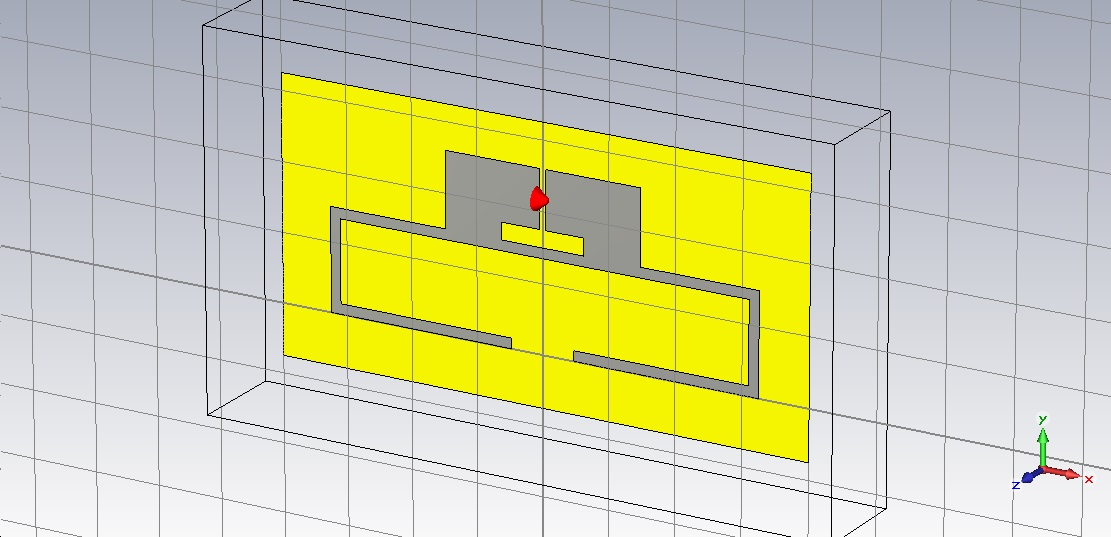
\includegraphics[width=16cm]{struktura_plaska.jpg}
	    \caption{Model struktury anteny w programie \emph{CST Microwave Studio}}
\end{figure}

\newpage
\begin{table}[h!]
\begin{center}
    \begin{tabular}{|c|c|}
    \hline
    ~                 & ~       \\
    PARAMETR          & WARTOŚĆ \\
    ~                 & ~       \\ \hline
    ~                 & ~       \\
    L                 & 130 mm  \\
    ~                 & ~       \\ \hline
    ~                 & ~       \\
    L1                & 55.5 mm \\
    ~                 & ~       \\ \hline
    ~                 & ~       \\
    L2                & 59 mm   \\
    ~                 & ~       \\ \hline
    ~                 & ~       \\
    H                 & 30 mm   \\
    ~                 & ~       \\ \hline
    ~                 & ~       \\
    H2                & 22 mm   \\
    ~                 & ~       \\ \hline
    ~                 & ~       \\
    D                 & 5 mm    \\
    ~                 & ~       \\ \hline
    ~                 & ~       \\
    D2                & 2 mm    \\
    ~                 & ~       \\ \hline
    ~                 & ~       \\
    W                 & 3 mm    \\
    ~                 & ~       \\ \hline
    ~                 & ~       \\
    W2                & 17 mm   \\
    ~                 & ~       \\ \hline
    ~                 & ~       \\
    DLUGOŚĆ PODŁOŻA   & 15.5 mm \\
    ~                 & ~       \\ \hline
    ~                 & ~       \\
    SZEROKOŚĆ PODŁOŻA & 7.5 mm  \\
    ~                 & ~       \\ \hline
    \end{tabular}
	\caption{Wymiary struktury anteny}
\end{center}
\end{table}


Wykonana antena tekstylna ma strukturę dipola z układem dopasowującym. Podłoże wykonano z papieru (aby struktura anteny była elastyczna i giętka, a co za tym idzie możliwe było jej przymocowanie na ramieniu człowieka).Przenikalność elektryczną podłoża przyjęto jak dla papieru $\epsilon_{r}$ = 2.31.

\noindent
\newline

 
\newpage
\section{Struktura anteny tekstylnej}

W programie \emph{CST Microwave Studio} zaprojektowano  model anteny tekstylnej naramiennej. Do celów symulacji dla modelu ramienia przyjęto zgodnie z artykułem KKRRiT z 2013 roku \cite{Artykul_1}  $\epsilon_{r}$ = 52 i $\sigma$ = 1,8.

\begin{figure}[!ht]
	\centering
	    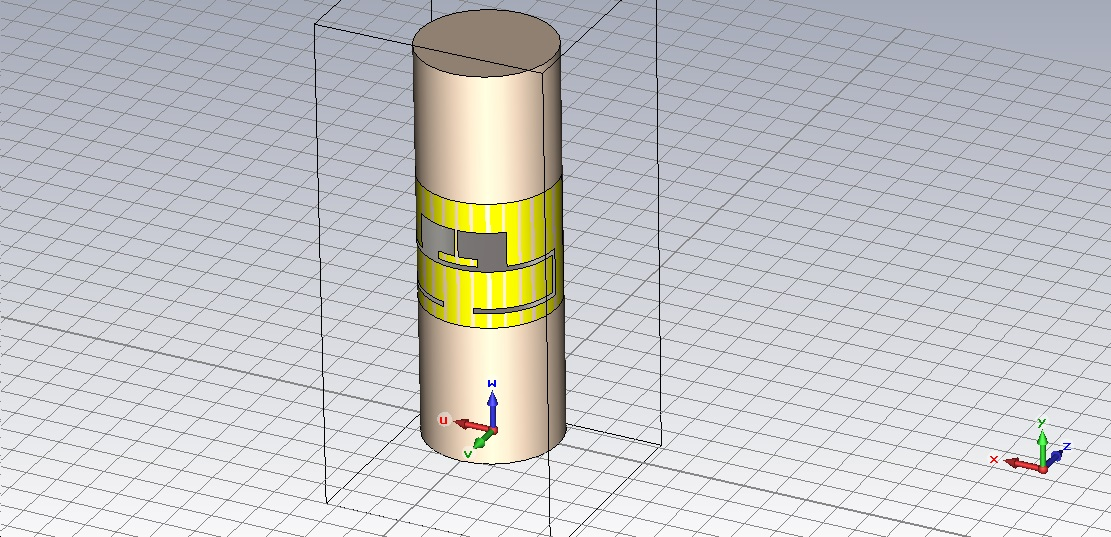
\includegraphics[width=16cm]{struktura_ramie.jpg}
	    \caption{Model struktury anteny tekstylnej naramiennej z programu \emph{CST Microwave Studio}}
\end{figure}

\newpage
\begin{figure}[!th!]
	\centering
	    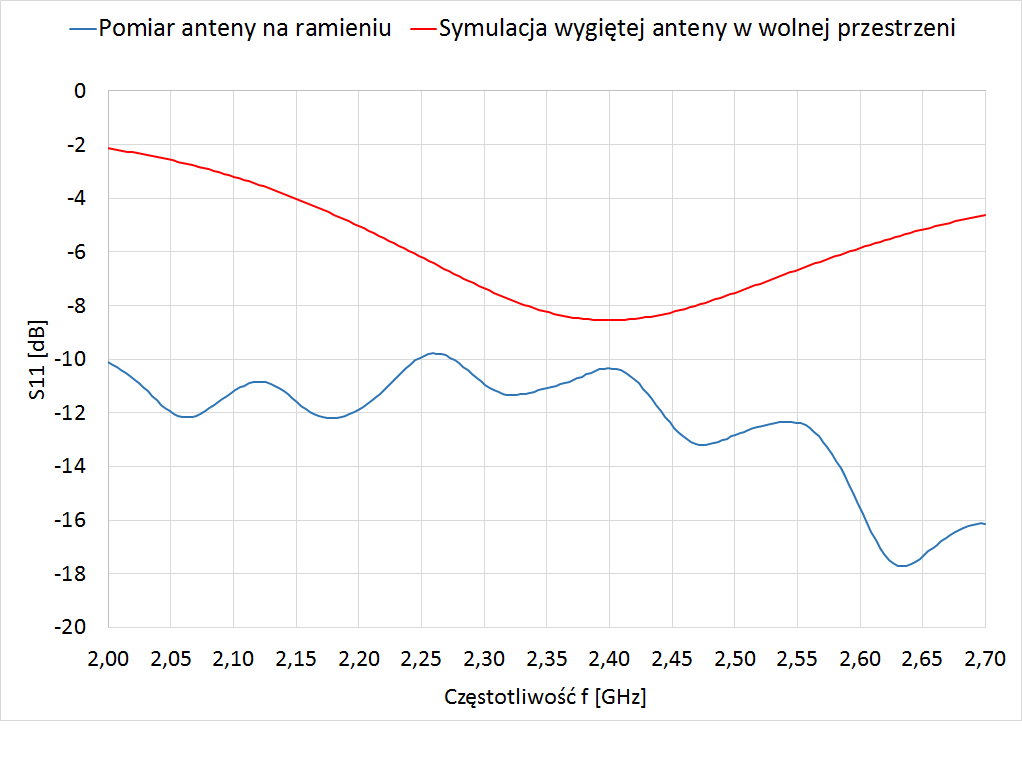
\includegraphics[width=16cm]{POM_Ram_SYM_Pow.jpg}
	    \caption{Przebieg zależności parametru $s_{11}$ od częstotliwośći dla pomiaru anteny na ramieniu, porównany z wynikami symulacji anteny wygiętej w wolnej przestrzeni}   
\end{figure}


\chapter{Wyniki pomiarów}

\section{Pomiar i porównanie parametru $s_{11}$}

Pomiar parametru rozproszenia $s_{11}$ został przeprowadzony analizatorem widma firmy Agilent typu N5230A. Następnie otrzymane wyniki zostały porównane z wynikami symulacji uzyskanymi w programie \emph{CST Microwave Studio}. Jak widać na Rys. 5.1 wynik pomiaru różnił się od wyników symulacji. W trakcie pomarów na kabel zasilający antenę zostały nałożone koraliki ferrytowe, aby zmniejszyć do minimum promieniowanie kabla i ewentualne zakłócenia z tym związane. 


\begin{figure}[h!]
\centering
	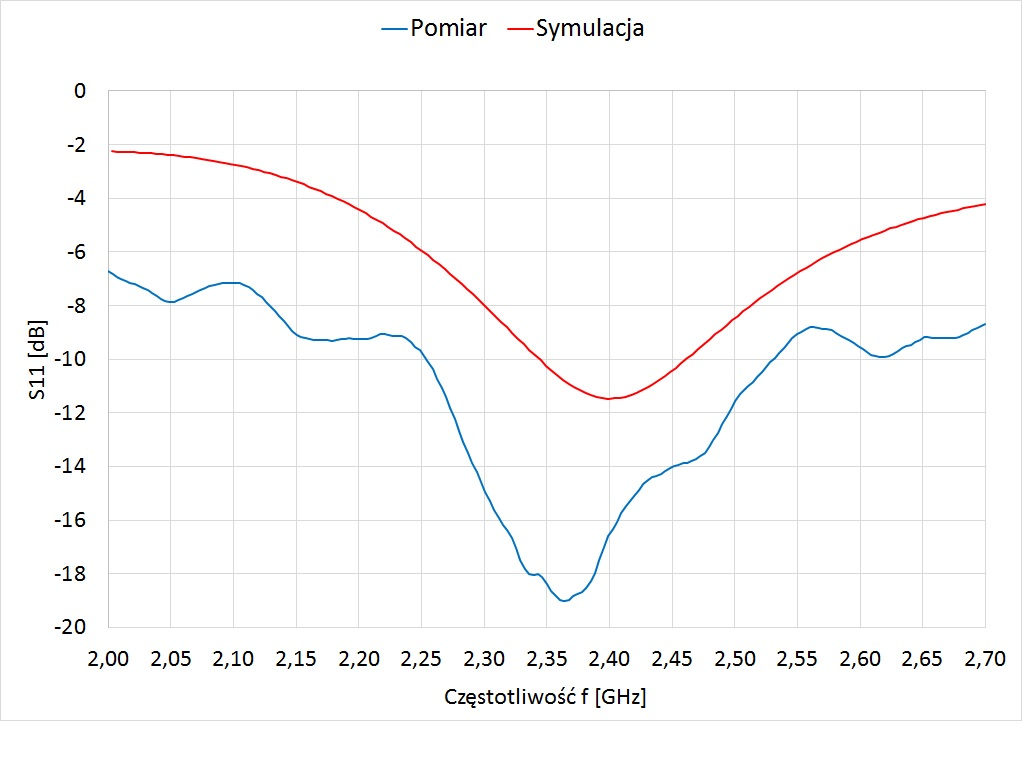
\includegraphics[width=16cm]{POM_Prz_Ko_SYM_Prz_Ko.jpg}
	\caption{Wykres zależności parametru $s_{11}$ od czestotliwości dla anteny przed korektą, porównany z wynikami symulacji}
\end{figure}


\newpage
Dla celów symulacji przyjęto przenikalność elektryczną podłoża równą $\epsilon_{r}$ = 2.31. Strukturę podano modyfikacji, aby poprawić jej częstotliwości pracy. Wprowadzone zmiany polegały na skróceniu długości ramion dipola, o około 5 mm tak aby mogła ona pracować na częstotliwośći 2,4 GHz. Zauważyć można, że przed modyfikacją ramion dipola częstotliwosć pracy anteny wynosiła \emph{F=2,364 GHz}, natomiast po modyfikacji \emph{F=2,3654 GHz} (patrz Rys.5.2 i Rys. 5.3).  

\begin{figure}[h!]
\centering
	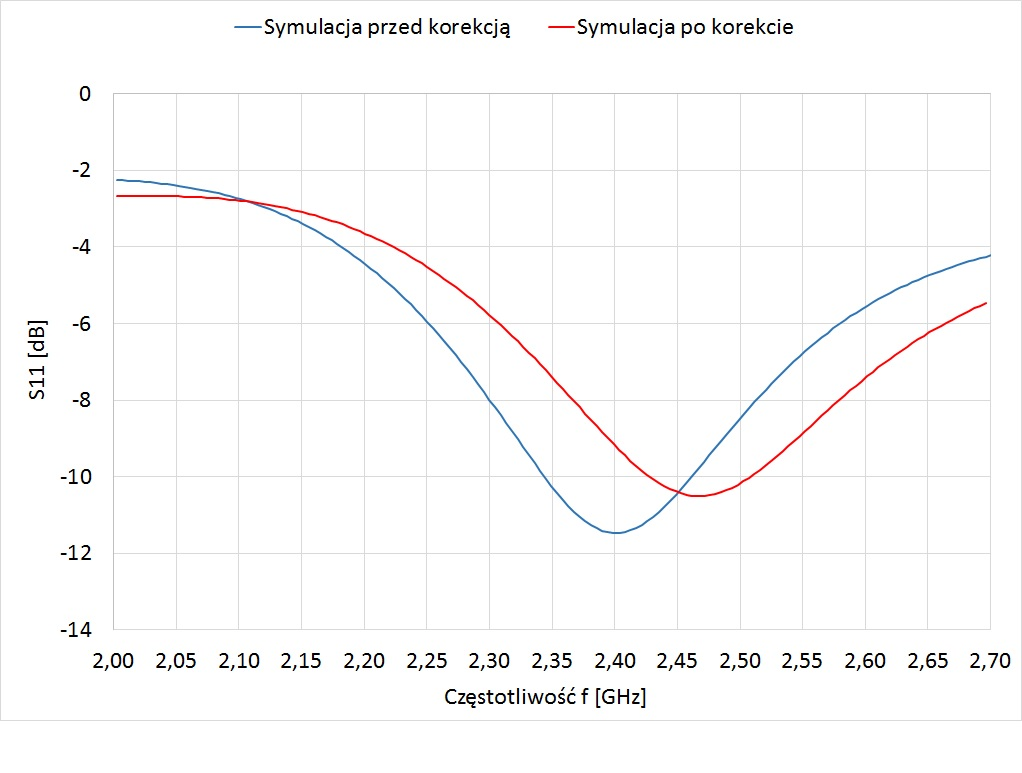
\includegraphics[width=16cm]{SYM_Prz_Ko_SYM_Po_Ko.jpg}
	\caption{Przebieg zależności parametru $s_{11}$ od czestotliwości dla symulacji przed korekcją porównany z symulacją anteny po korekcji}
\end{figure}


\begin{figure}[h!]
\centering
	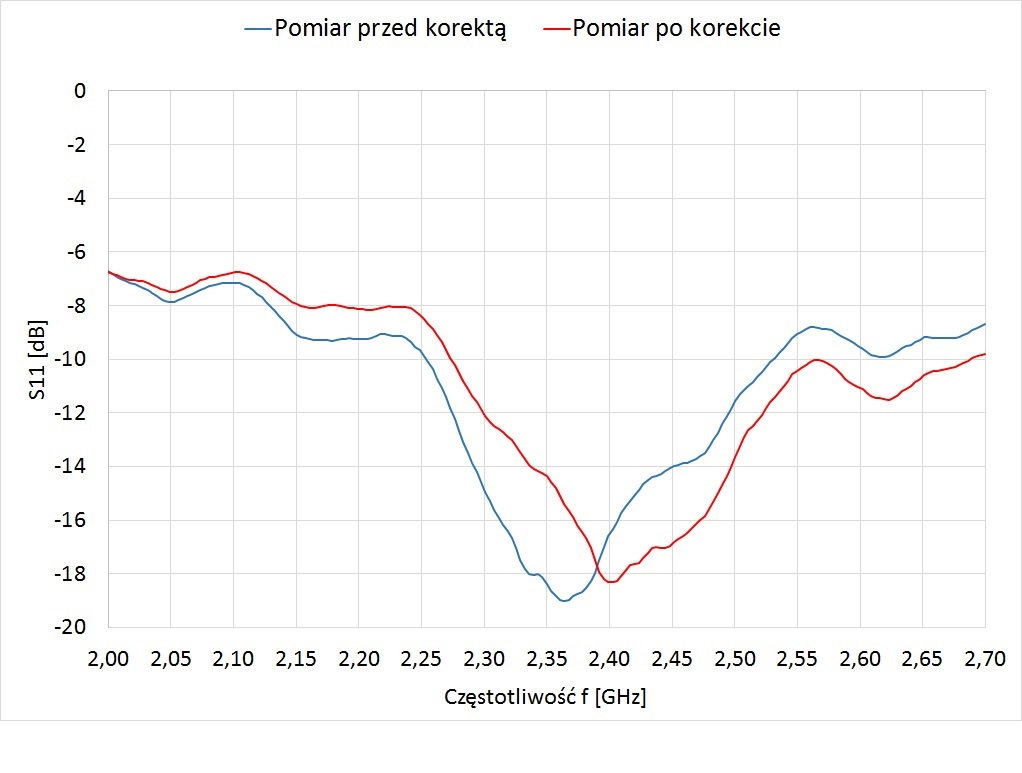
\includegraphics[width=16cm]{POM_Prz_Ko_POM_Po_Ko.jpg}
	\caption{Przebieg zależności parametru $s_{11}$ od czestotliwości dla anteny przed korektą porównany z wynikami anteny po korekcie}
\end{figure}


\newpage
\noindent
\newline Umieszczenie anteny na ramieniu człowieka spowodowało przesunięcie częstotliwości rezonansowej w "góre", która wynosi dla tego przypadku \emph{F=2,6349 GHz} (patrz Rys. 5.4). Wynika to z faktu, iż parametry anten silnie zależą od właściwości ośrodka stratnego.  
Tkanka ludzka jest dielektrycznym, dyspersyjnym ośrodkiem stratnym o skończonej konduktywności. Ponaddto fale o takiej samej częstotliwośći (w ośrodku dyspersyjnym), rozchodzą się z różną prędkością. 

\begin{figure}[h!]
\centering
	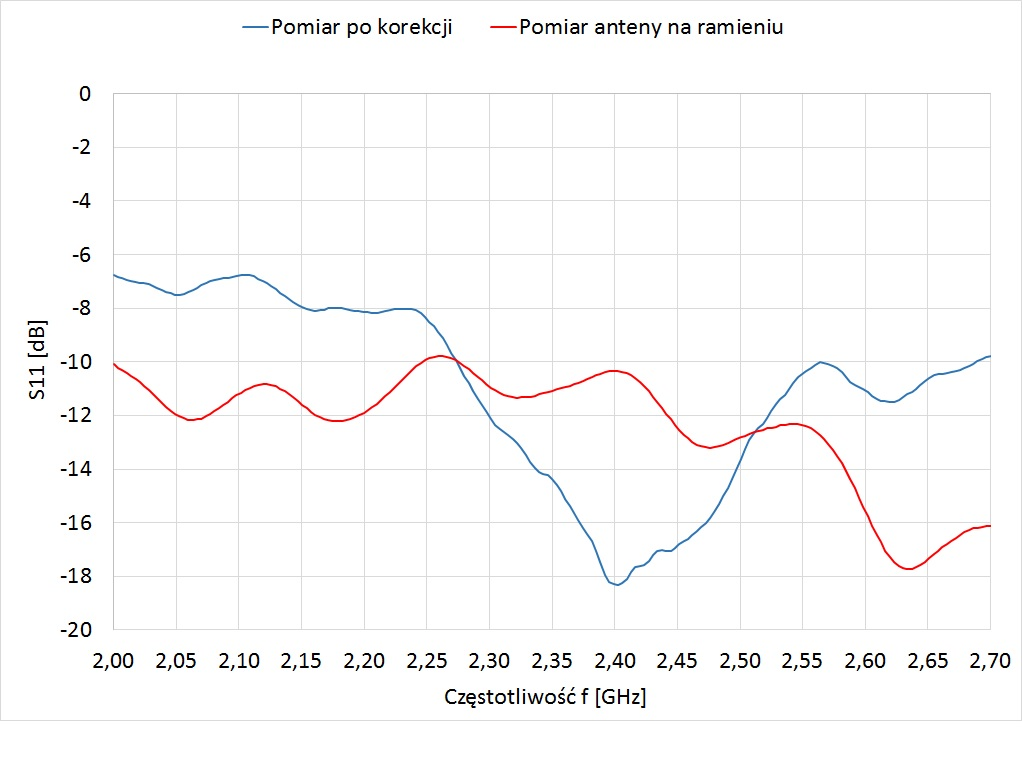
\includegraphics[width=16cm]{POM_Po_Ko_POM_Ram.jpg}
	\caption{Wykres zależności parametru $s_{11}$ od czestotliwości dla anteny po korekcji, porównany z pomiarami anteny umieszczonej na ramieniu}
\end{figure}


\newpage

\section{Zysk energetyczny}

Do pomiaru zysku energetycznego wybrano metodę porównawczą.

\subsection {Metoda porównanwacza}

Do pomiaru zysku energetycznego wybrano metodę porównawczę, którą zaczerpnięto ze skryptu wydanego przez Oficynę Wydawniczą Politechniki Śląskiej \emph{Pomiary parametrów anten} \cite{Pomiary_parametrów}. Układ pomiarowy składał się z anteny nadawczej  i anteny odbiorczej (anteny wzorcowej / badanej). Przyjęto założenie, że warunki pomiaru są niezmienne w czasie: zysk anteny nadawczej jest stały, poziom mocy sygnału emitowanego przez antenę nadawczą jest stały oraz odległość anteny nadawczej od anteny odbiorczej jest stała. Na podstawie zysk energetycznego anteny wzorcowej, który jest znany i dla częstotliwości 2,4 GHz wynosi 10.24 dB, zmierzyliśmy zysk anteny badanej. Antenę nadawczą podłączono do generetora funkcyjnego 
Rohde\&Schwarz SMF 100A i ustawiono jego częstotliwość pracy na 2,4 GHz. W polu promieniowania anteny nadawczej umieszczono antenę odbiorczą (badaną), którą podłączono do analizatora widma \& Agilent N5230A i wybrano odpowiedni zakres pracy analizatora. Po ustawieniu częstotliwości nadawania dokonano pomiaru poziomu mocy odebranej przez antenę wzorcową za pomocą analizatora widma. Następnie w miejscu anteny wzorcowej, na tej samej wysokości i w niezmienionej odległości od anteny nadawczej, umieszczono antenę RFID, dla której zmierzono poziom mocy odbieranej. 


\noindent
\newline Uzyskane wyniki pomiarów poziomu mocy zestawiono w tabeli 5.1:


\begin{table}[h!]
\begin{center}
    \begin{tabular}{|c|c|c|}
    \hline
    ~                     & ~               & ~                         \\
     RODZAJ POLARYZACJI    & ANTENA WZORCOWA & ANTENA MIERZONA TEKSTYLNA \\
    ~                     & ~               & ~                         \\ \hline
    ~                     & ~               & ~                         \\
     POLARYZACJA POZIOMA  & -34.5 dBm       & -39,2 dBm                 \\
    ~                     & ~               & ~                         \\ \hline
    ~                     & ~               & ~                         \\
     POLARYZACJA PIONOWA  & -59.7 dBm       & -59.9 dBm                 \\
    ~                     & ~               & ~                         \\ \hline
    \end{tabular}
    \caption{Poziom mocy sygnału}
\end{center}
\end{table}


\noindent
\newline Uzyskane wyniki pomiarów zysku energetycznego zestawiono w tabeli 5.2:


\begin{table}[h!]
\begin{center}
    \begin{tabular}{|c|c|c|c|}
    \hline
    ~               & \multicolumn{3}{c|}{~}     \\
    ~               & \multicolumn{3}{c|}{ANTENA MIERZONA TEKSTYLNA } \\
    ~               & \multicolumn{3}{c|}{~}     \\ \hline
    ~               & \multicolumn{2}{c|}{~}     & ~                                  \\
    ANTENA WZORCOWA & \multicolumn{2}{c|}{BEZ OBECNOŚCI CZŁOWIEKA} & W OBECNOŚCI CZŁOWIEKA              \\
    ~               & \multicolumn{2}{c|}{~}     & ~                                  \\ \hline
    ~               & ~                          & ~                                  & ~                                  \\
    ~               & POŁOŻENIE ----             & POŁOŻENIE [     ]                  & POŁOŻENIE [    ]                   \\
    ~               & ~                          & ~                                  & ~                                  \\ \hline
    ~               & ~                          & ~                                  & ~                                  \\
    -10.24 dB       & -38.25 dB                  & -46.05 dB                          & -49.04 dB                          \\
    ~               & ~                          & ~                                  & ~                                  \\ \hline
    \end{tabular}
    \caption{Zysk energetyczny badanych anten}
\end{center}
\end{table}


\noindent
\newline Zysk anteny tekstylnej RFID $G_{RFID}[dBi]$  wyznaczono, koszytając z poniższego wzoru:

\begin{align}
G_{RFID}[dBi] = G_{W}[dBi] + P_{RFID}[dBm] - P_W[dBm]
\quad
\end{align}


\noindent
\newline gdzie: 

\noindent
\newline$G_{RFID}[dBi]$ - zysk anteny RFID w odniesieniu do anteny izotopowej, 


\noindent
\newline $G_{W}[dBi]$ - zysk anteny wzorcowej w odniesieniu do anteny izotopowej (podany przez producenta),

\noindent
\newline $P_{RFID}[dBm]$ - poziom mocy sygnału odebrany przez antenę RFID,


\noindent
\newline $P_W[dBm]$ - poziom mocy sygnału odebrany przez antenę wzorcową.

\noindent
\newline Zysk energetyczny dla częstotliwości 2,4 GHz dla polaryzacji poziomej:

\begin{align}
G_{RFID}[dBi] = 10.24[dBi] - 39.2[dBm] + 34.5[dBm] = 5,54[dBi]
\quad
\end{align}




W trakcie pomiarów założono, że obie anteny odbiorcze są dopasowene. Względna różnica poziomu mocy odebranej przez antenę badaną i abntenę wzorcową pozwala określić wartość zysku energetycznego anteny badanej. Wyniki obarczone są pewnymi błędami, co wynika z faktu nieidealności samej metody pomiarowej oraz warunków w jakich przeprowadzany był pomiar. Pomiary nie były przeprowadzone w wolnej przestrzeni, ale w budynku wydziału Automatyki, Elektroniki i Informatyki.

\newpage
\section{Charakterystyka promieniowania}
Wykresy pokazane na Rys. 5.5 i Rys. 5.6 przedstawiają charakterystyki promieniowania anteny w biegunowym układzie współrzędnych w płaszczyźnie $\phi = 90^{0}$ natomiast wykres na Rys. 5.7 pokazuje trójwymiarową charakterystkę promieniowania zamodelowanej anteny RFID dla częstotliwości 2.4 GHz.


\begin{figure}[h!]
\centering
	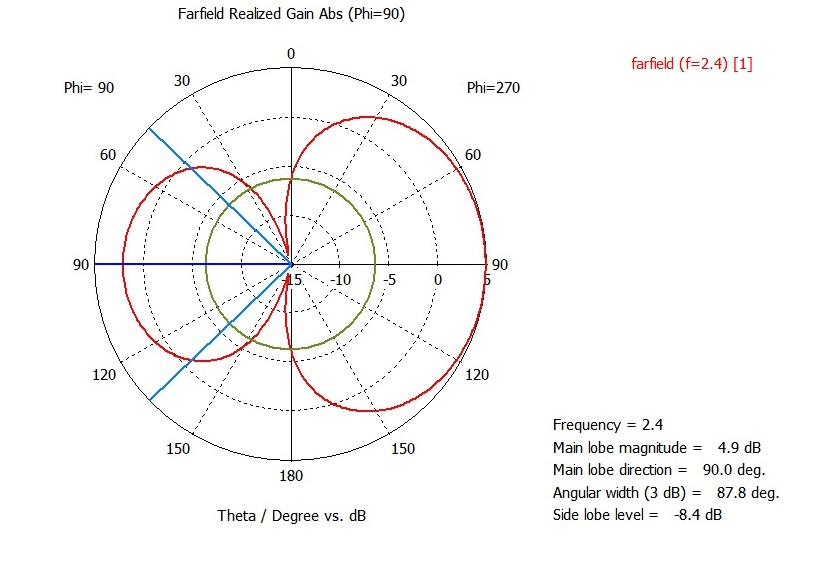
\includegraphics[width=15cm]{Gain_Abs_90.jpg}
	\caption{Przebieg charakterystyki promieniowania anteny w płaszczyźnie $\phi = 90^{0}$}
\end{figure}

\noindent
\newline

\begin{figure}[h!]
\centering
	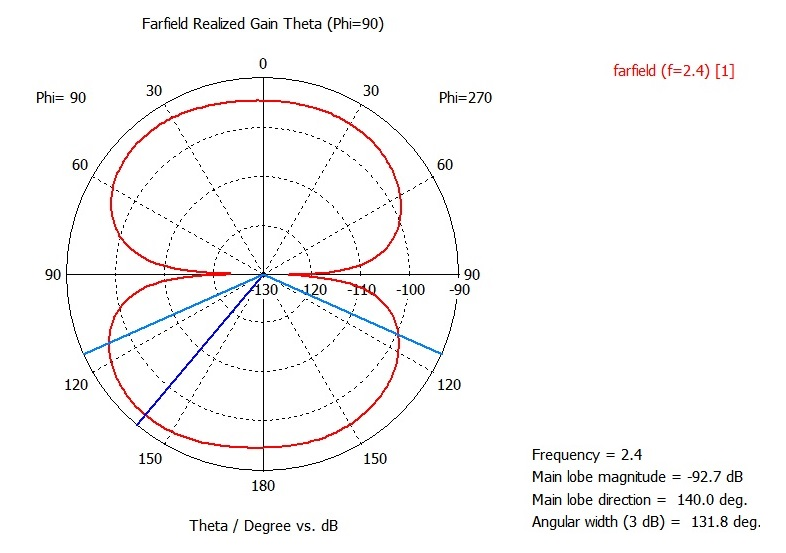
\includegraphics[width=15cm]{Gain_Theta_90.jpg}
	\caption{Przebieg charakterystyki promieniowania anteny w płaszczyźnie $\phi = 90^{0}$}
\end{figure}

\noindent
\newline

\begin{figure}[h!]
\centering
	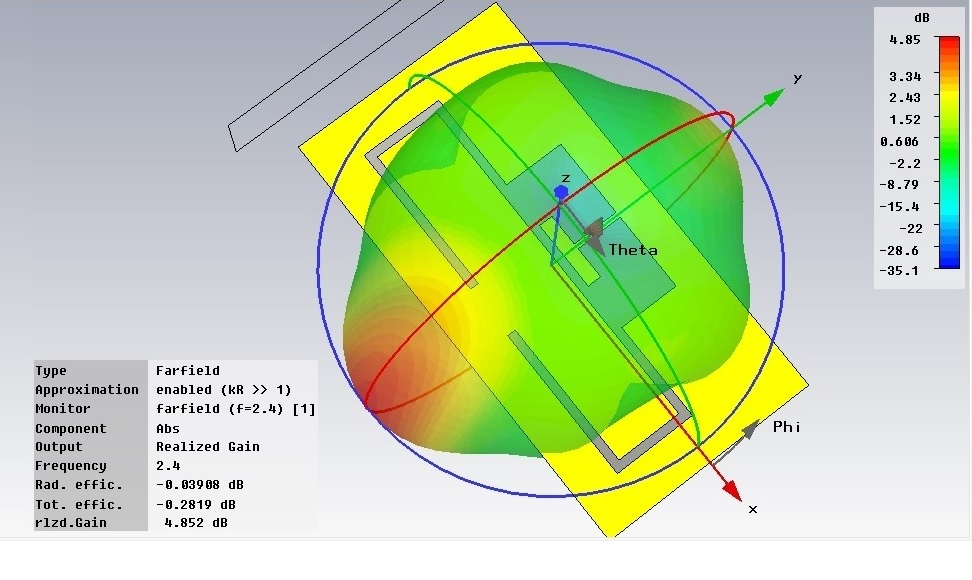
\includegraphics[width=16cm]{Abs.jpg}
	\caption{Charakterystyka 3D promieniowania anteny dla częstotliwości 2,4 GHz}
\end{figure}





\newpage
\noindent
\newline

\section{Impedancja}



Wykresy (patrz Rys. 5.8 i Rys 5.9) przedstawiają zależność impedancji od częstotliwości. 
\newline Impedancja wejściowa zamodelowanej w programie anteny wynosi 38 \(\Omega\).

\begin{figure}[h!]
\centering
	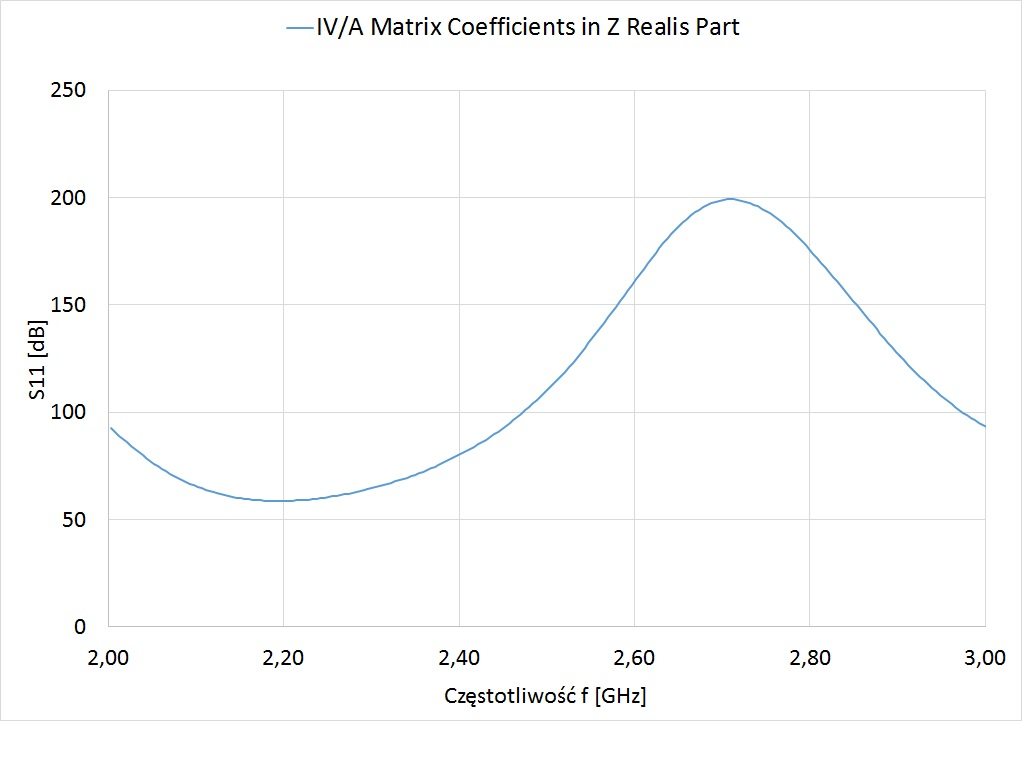
\includegraphics[width=16cm]{AN_PL_Z_REAL.jpg}
	\caption{Wykres zależności części rzeczywistej impedancji anteny od częstotliwości}
\end{figure}

\newpage
\begin{figure}[h!]
\centering
	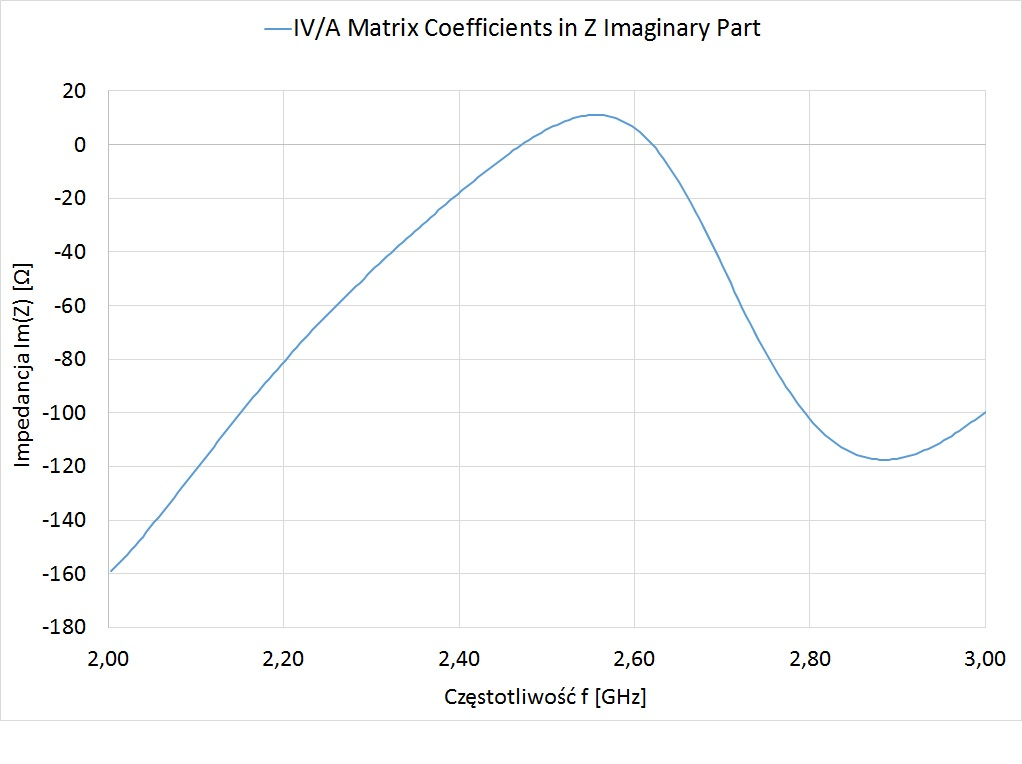
\includegraphics[width=16cm]{AN_PL_Z_IMAG.jpg}
	\caption{Wykres zależności cześci urojonej impedancji anteny od częstotliwości}
\end{figure}




\newpage
Wykresy (patrz Rys. 5.10 i Rys 5.11) przedstawiają zależność impedancji od częstotliwości. 
%\begin{figure}[h!]
%\centering
%	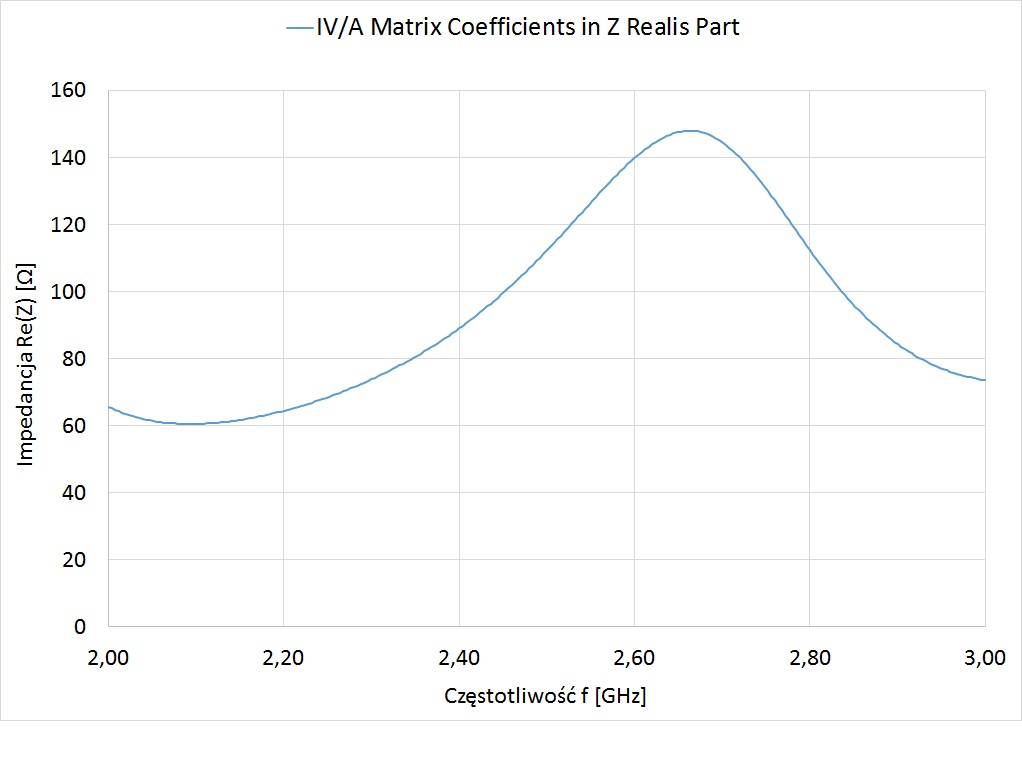
\includegraphics[width=16cm]{AN_WYG_Z_REAL.jpg}
%	\caption{Wykres zależności części rzeczywistej impedancji anteny na modelu ramienia od częstotliwości}
%\end{figure}

%\newpage
%\begin{figure}[h!]
%\centering
%	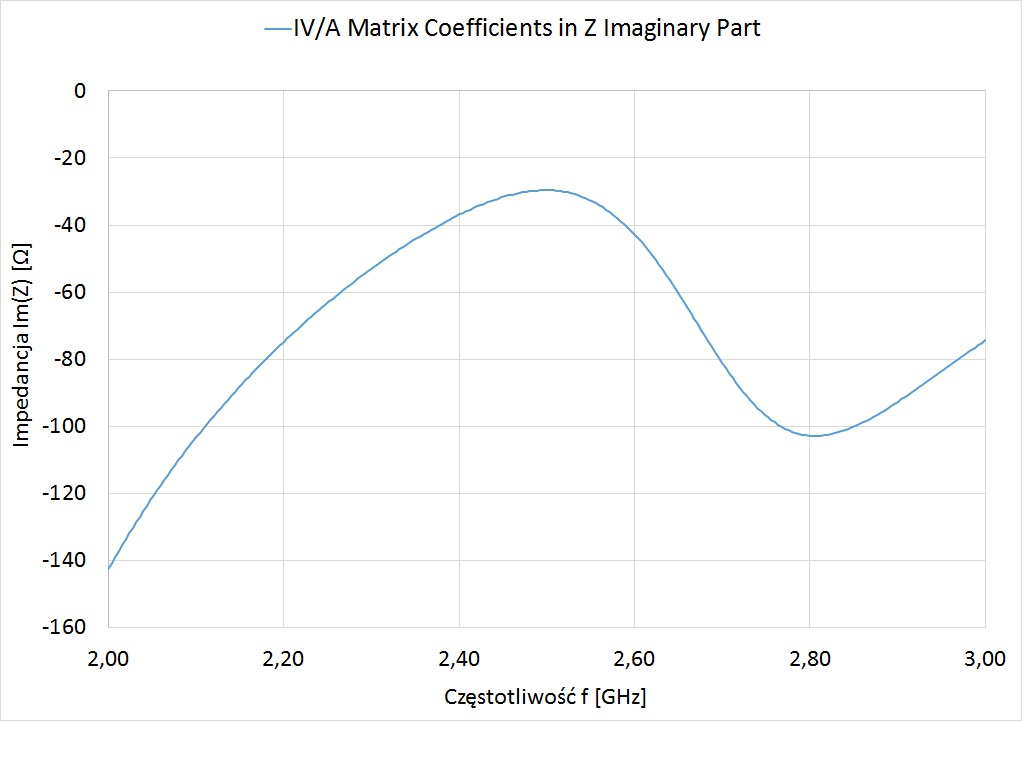
\includegraphics[width=16cm]{AN_WYG_Z_IMAG.jpg}
%	\caption{Wykres zależności cześci urojonej impedancji anteny na modelu ramienia od częstotliwości}
%\end{figure}



\newpage
Wykresy (patrz Rys. 5.12 i Rys 5.13) przedstawiają zależność impedancji od częstotliwości dla anteny umieszczonej na modelu ramienia. Dla\cite{Artykul_1}  $\epsilon_{r}$ = 52 i $\sigma$ = 1,8.
\begin{figure}[h!]
\centering
	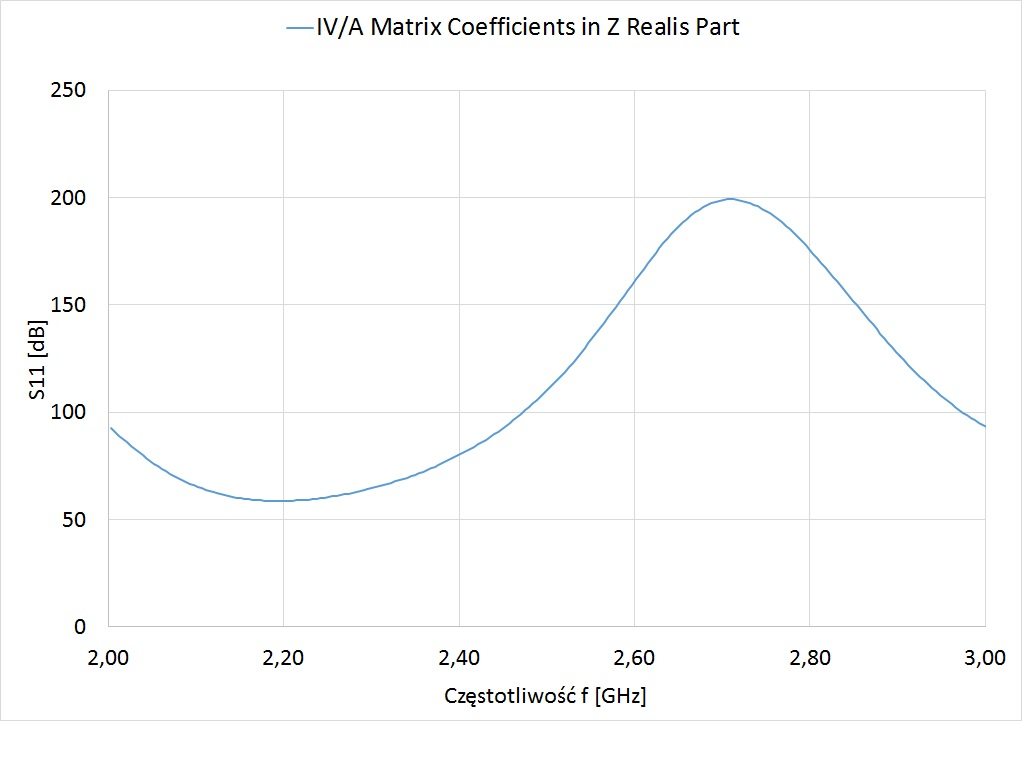
\includegraphics[width=16cm]{AN_RAM_Z_REAL.jpg}
	\caption{Wykres zależności części rzeczywistej impedancji anteny umieszczonej na modelu ramienia od częstotliwości}
\end{figure}


\newpage
\begin{figure}[h!]
\centering
	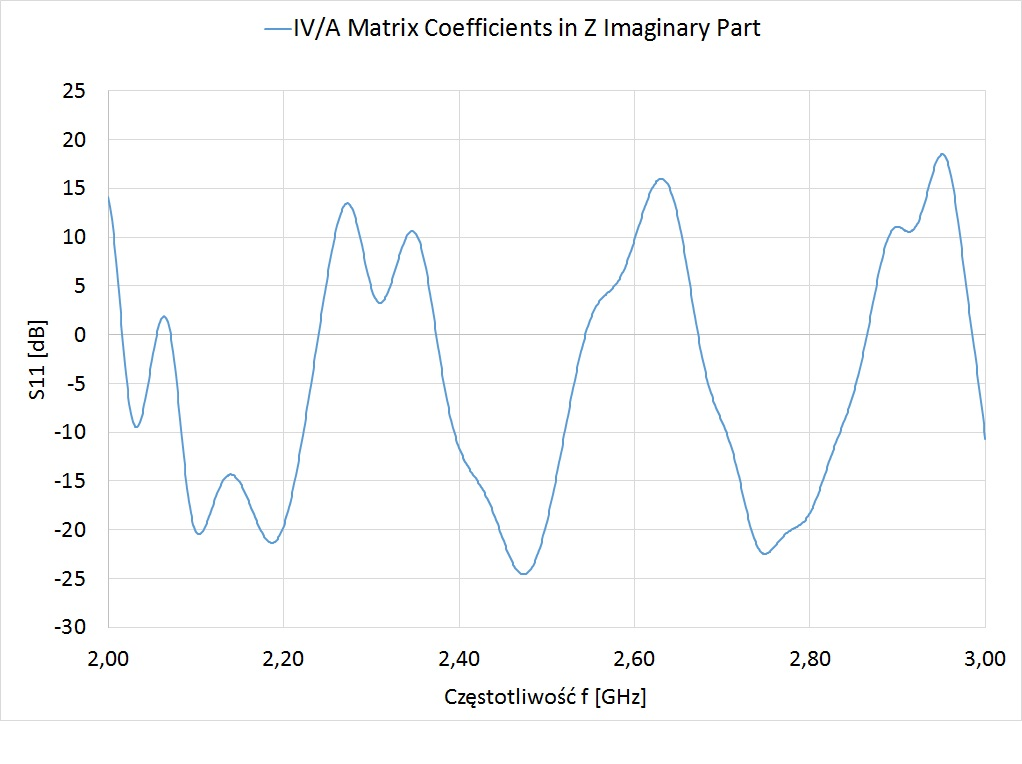
\includegraphics[width=16cm]{AN_RAM_Z_IMAG.jpg}
	\caption{Wykres zależności cześci urojonej impedancji anteny umieszczonej na modelu ramienia od częstotliwości}
\end{figure}


\chapter{Podsumowanie}

Celem pracy inżynierskiej było zaprojektowanie anteny tekstylnej pracującej na częstotliwości 2,4 GHz. Anteny tekstylne należą do grupy anten konforemnych, trudnych technologicznie do wykonania ze względu na elastyczność podłoża, prace w trudnych warunkach, konieczność integracji z nośnikiem (kamizelką, rękawem, kaskiem) jednak mających coraz szersze zastosowanie. W ciągu ostatnich lat zwiększa się zapotrzebowanie na tego typu anteny przytwierdzone do fragmentów odzieży.
Projekt anteny wykonano w środkowisku \emph{CST Microwave Studio}. W pierwszej fazie zamodelowano i przesymulowano zmodyfikiwoną strukturę anteny zaprezentowaną w artykule \cite{Artykul_1}. Celem poprawy parametrów anteny zmodyfikowano o kilka milimetrów wymiary struktury wzorcowej (patrz Rys. 4.2, 4.3 i Tab. 4.1). Wprowadzone modyfikacje dwukrotnie zwiększyły zysk, zmniejszyły impedancję wejściową prawie trzykrotnie i dostroiły częstotliwość anteny do nominalnej częstotliwości pracy.
Strukturę anteny początkowo zamodelowano na niezdeformowanym (płaskim) podłożu, a następnie je wygięto w tych w obydwu przypadkach antenę umieszczono w ośrodku o $\epsilon_{r}$ = 1 (powietrze), w kolejnej fazie symulacji antenę umieszczono na modelu ramienia o $\epsilon_{r}$ = 52 (ośrodek stratny).    
Dla zaprojektowanej anteny zmierzono parametr $s_{11}$, poziom mocy sygnału odebranego i zysk energetyczny. Największe rozbieżności na wykresach można zaobserwować dla pomiaru zysku energetycznego dla anteny mierzonej w na płasko i anteny umieszczonej na ramieniu (patrz rys. 5.4). Zysku anteny spadł o około 8 dB dla anteny umieszczonej na ramieniu (dla częstotliwości 2,4 GHz), co jest niewątpliwie wynikiem deformacji całej struktury jak i zmiany ośrodka pracy. 
Przeprowadzone pomiary podstawowych parametrów anteny tekstylnej w środowisku rzeczywistym pokazały w jaki sposób obecność ludzkiego ciała wpływa na charakterystykę promieniowania anteny i jej zysk.
Strukturę anteny można poddać dalszym modyfikacją, aby jej parametry polowe jeszcze się poprawiły. Papierowe podłożę można zastąpić podłożem z materiału, a miedzianą strukturę, nićmi z przewodzącymi włóknami wtedy z powoedzeniem powdzeniem możnaby umieścić wykonaną antenę RFID wewnątrz odzieży, gdyż nie ogranicza swobody ruchu człowieka i nie wywołuje uczucia dyskomfortu ze względu na elastyczne podłoże.